\chapter{概要设计}

% 本章主要阐述了系统架构、系统各模块具体架构和数据库概要设计等方面的内容,通过借助系统结构图和活动图来描述各功能实现的基本原理,为第五章的详细设计奠定了基础。

本章对系统的整体架构、系统各功能模块的详细架构以及数据库概要设计等方面的内容作了细致的阐述,通过系统结构图与活动图来说明各功能实现的基本原理,为第五章系统的详细设计打下了基础。


\section{系统架构设计}

根据微服务的拆分原则,可将系统的功能拆分为四大模块,分别是存储管理模块、权限控制模块、认证中心模块和API网关模块。系统整体的逻辑架构如图\ref{fig:系统逻辑架构图}所示。
\begin{figure}[h]
    \centering
    \includegraphics[width=0.8\textwidth]{my_figures/chapter4/系统逻辑架构图.png}
    \caption{系统逻辑架构图}
    \label{fig:系统逻辑架构图}
%     \note{注:图注的内容不宜放到图题中。}
\end{figure}

根据上面的系统逻辑架构图,可以看到存储管理、权限控制和认证中心这三个微服务都是通过API网关与前端进行交互,API网关就相当于大门,网关微服务也是整个系统对外暴露的
唯一端口。当请求访问到网关微服务的端口时,首先要做的是去认证中心进行身份校验,确保用户信息的准确性。而权限控制模块则主要负责管理用户的账号、角色和权限等信息。
存储管理平台模块是整个管控系统的核心服务模块,同时也与MySQL数据库和对象存储系统服务器相连接,MySQL数据库中主要存储管控平台上使用者的帐号、角色和权限等有关信息,
对象存储系统服务器是用户上传或下载文件的位置,是整个系统最关键的部分。

\section{系统功能模块架构}

\begin{figure}[h]
    \centering
    \includegraphics[width=0.8\textwidth]{my_figures/chapter4/系统功能模块图.png}
    \caption{系统功能模块图}
    \label{fig:系统功能模块图}
%     \note{注:图注的内容不宜放到图题中。}
\end{figure}

基于软件工程中高内聚、低耦合的思想,将分布式对象存储系统管控平台按功能划分为注册认证、权限控制、策略控制、文件存取和系统监控等五个模块。每个模块都含有若干个功能子
模块,注册认证模块可划分为四个子模块,分别是包含用户注册子模块、密码认证子模块、颁发令牌子模块和认证令牌子模块。权限控制模块可划分为四个子模块,分别是账号角色权限
管理、角色分配子模块、请求转发与鉴权子模块、网关路由管理子模块。策略控制模块可划分为四个子模块,分别是用户管理子模块、分组管理子模块、策略管理子模块、策略分配子模
块。文件存取模块可划分为四个子模块,分别是桶管理子模块、文件上传子模块、文件下载子模块、文件共享子模块。系统监控模块可划分为三个子模块,分别是状态监测子模块、记录
跟踪子模块、告警通知子模块。系统的功能模块图如图 \ref{fig:系统功能模块图}所示。

可以看到,系统的功能模块图中对模块的划分与系统用例表中的划分并不是完全相对的,两者有一些细微的差别,因为系统用例表是结合用户需求的实际情况,根据用户需求表抽象
出的系统用例,而系统的功能模块图是从系统实现的角度出发,结合软件工程中项目开发的思想去对系统进行功能划分。以策略控制模块为例,系统要进入策略控制模块首先需要经过
注册认证模块,而对于策略控制过程来说,为实现管理系统的可扩展性,在管理系统底层将策略控制的步骤中也经过了大量的子流程,而这些子流程中依次使用了网关鉴权功能、注册认
证功能以及策略控制模块这三种功能,但用户并没有感觉到这些子过程的发生,这些访问过程对于用户来说是透明的。通常情况下,在系统用例表中的每一条用例的实现,都必须一个模块或几个
模块的共同配合下方可完成。

\section{系统各功能模块设计}

\subsection{注册认证模块}



\begin{figure}[h]
    \centering
    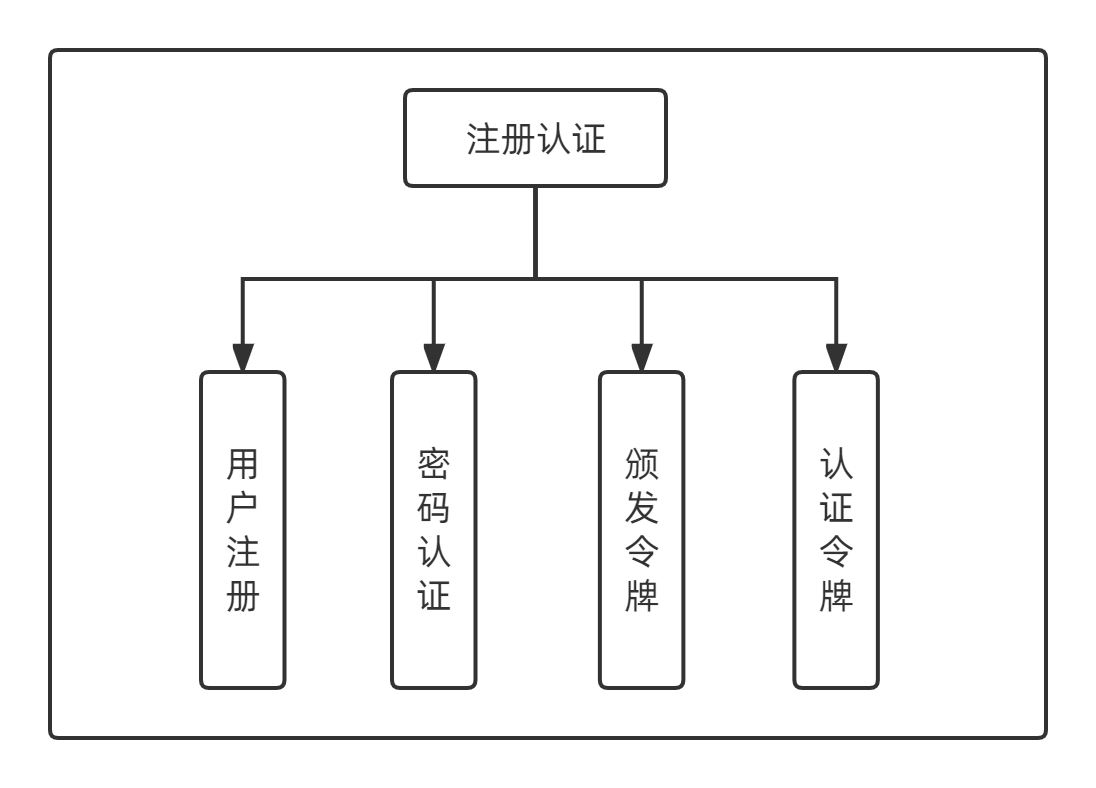
\includegraphics[width=0.5\textwidth]{my_figures/chapter4/注册认证模块功能结构图.png}
    \caption{注册认证模块功能结构图}
    \label{fig:注册认证模块功能结构图}
%     \note{注:图注的内容不宜放到图题中。}
\end{figure}

注册认证模块主要包含用户注册、密码认证、颁发令牌和认证令牌四个子功能模块。注册认证模块的功能结构图如图\ref{fig:注册认证模块功能结构图}所示。



(1)用户注册

本系统的登录用户一共有三种,分别是系统管理员、企业管理员和普通用户,其中系统管理员是不需要注册的,因为它会在项目部署初期由开发人员创建完成。
因此,需要进行用户注册的是企业管理员和普通用户。企业管理员由于身份特殊,在注册时会有一些特殊限制。

\begin{figure}[h]
    \centering
    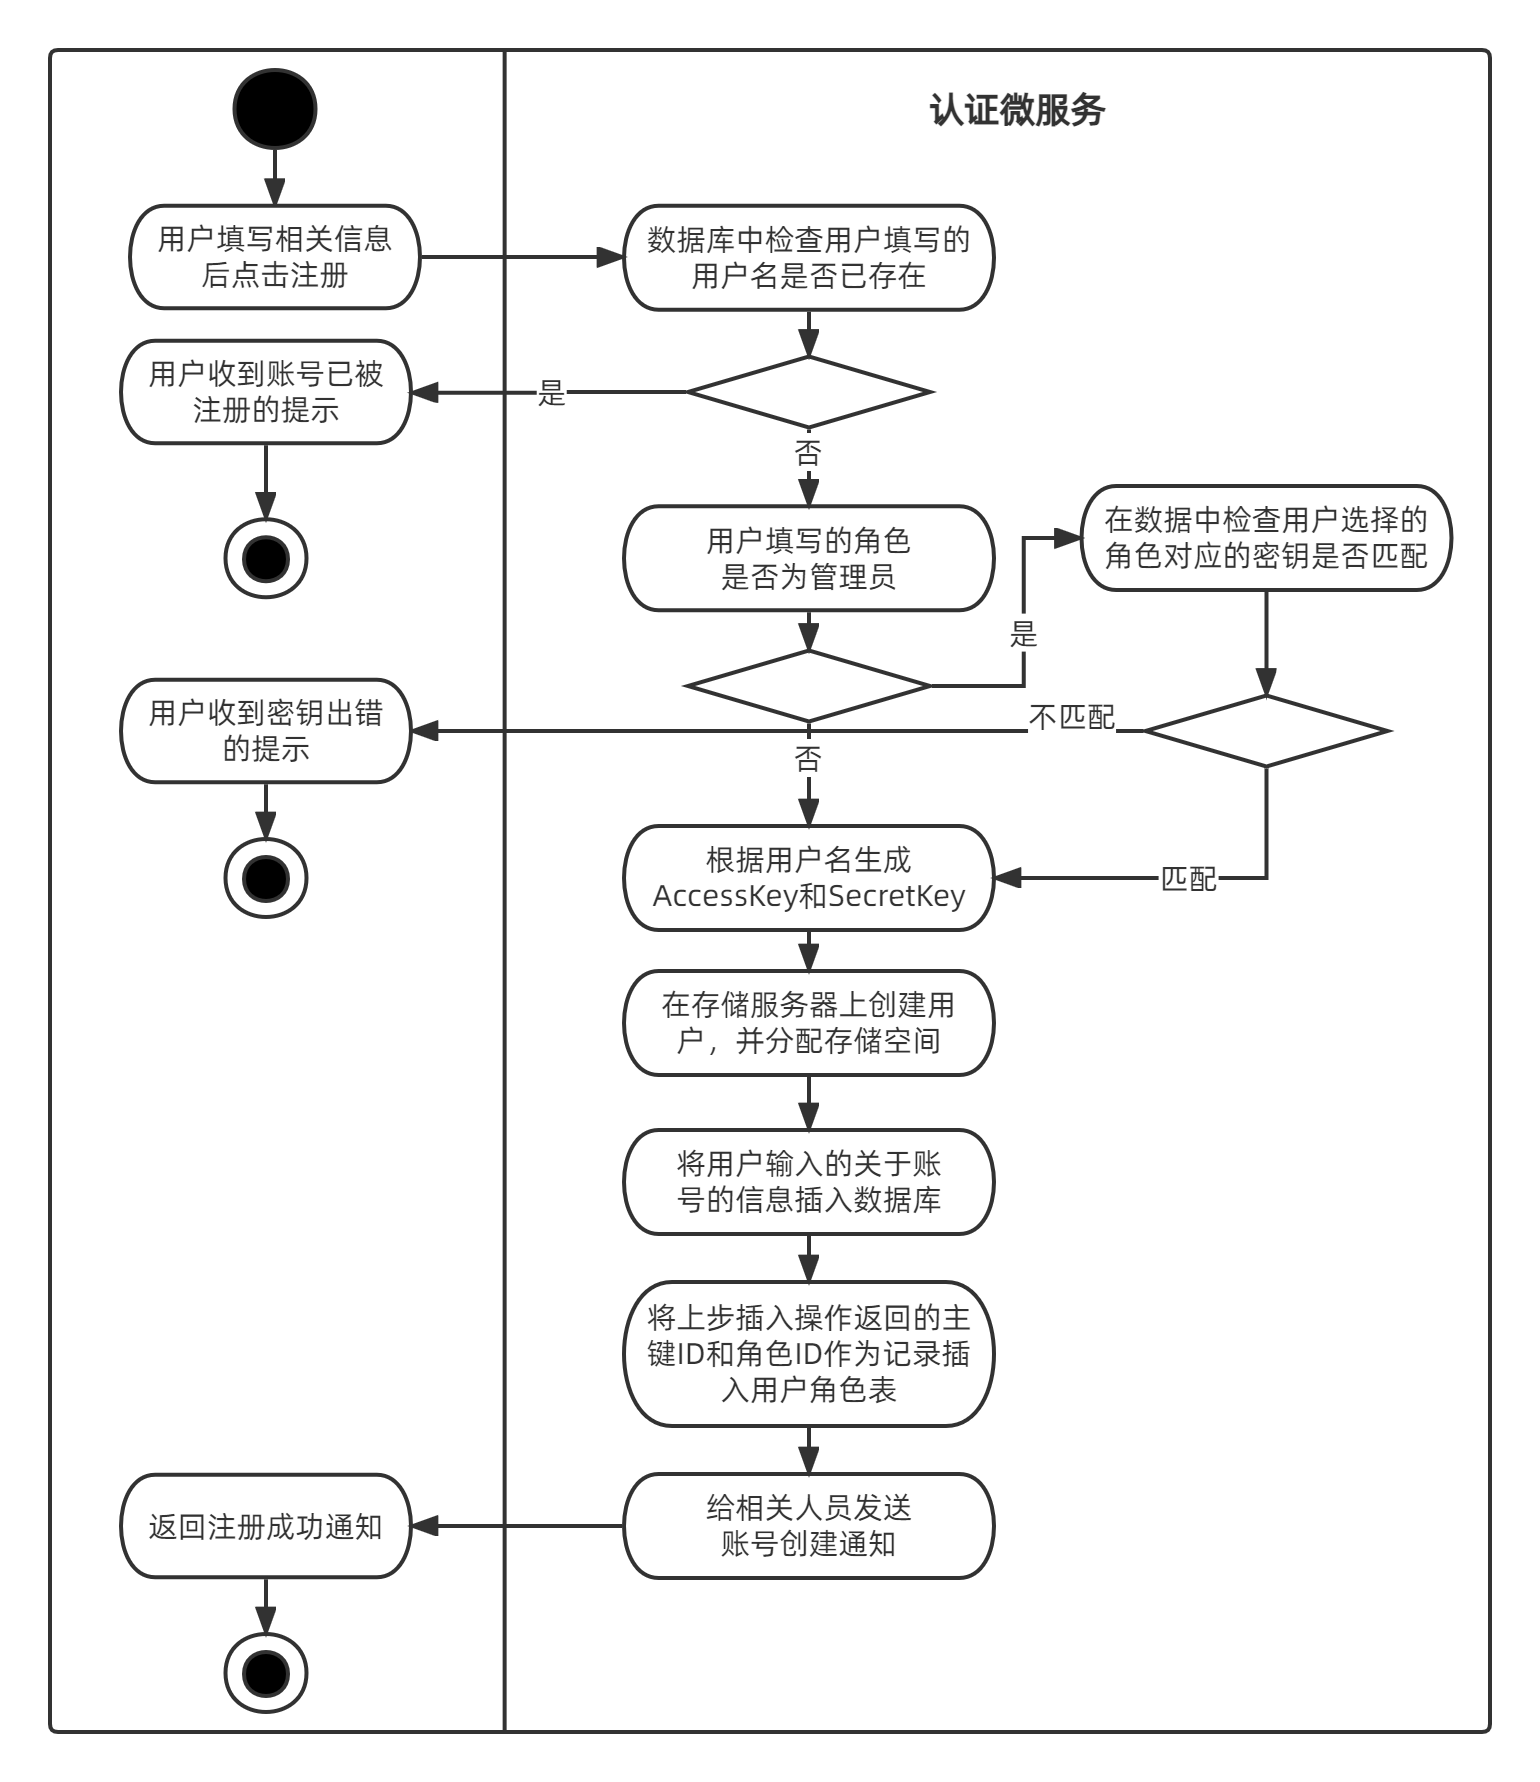
\includegraphics[width=0.7\textwidth]{my_figures/chapter4/用户注册活动图.png}
    \caption{用户注册活动图}
    \label{fig:用户注册活动图}
%     \note{注:图注的内容不宜放到图题中。}
\end{figure}

如果用户所注册的是企业管理员,用户在登录账
号时就必须选择企业管理员的角色,并准确的填写已提前向系统管理员申请的注册密钥,方能进行后续的注册流程,这样做的原因是为了避免外部人员非法获得
管理权限。

如果用户注册的是普通用户,用户在注册时不需要填写密钥,可直接进入后续的注册流程。
用户在注册时需要填写符合要求的用户名和密码,为了提
高账号的安全性,系统对密码的复杂度有一些要求,而且为了满足存储服务器用户名的要求,要求注册使用全英文的用户名。另外,企业管理员用户在注册时还
需要额外填写完整的企业信息和部分个人信息,以供系统管理员审核。


在提交注册信息后,系统首先会检查用户名是否存在,若用户名已存在,则会向前端报错,要求重新输入正确的用户名。在经过校验后,管理员用户或普通用户
都会根据用户名生成相应的AccessKey和 SecretKey,在远程存储服务器上创建对应的管理员用户和普通用户,且会为普通用户分配相应的存储空间。之后,
系统就会把所有用户输入的帐号信息进入数据库的用户列表中,将返回的主键ID与角色ID成为同一个记录,再插入到所有用户角色关联列表中。最后,会向系统
管理员和已注册用户发送用户创建的邮件通知,提示用户创建成功。用户注册活动图如图\ref{fig:用户注册活动图}所示。

(2)用户登录



用户在注册成功后会提示进入登录页面,用户填入已经注册成功的账号和密码,并选择角色,即企业管理员或普通用户。在登录请求发出后,系统后端会对用户名、
密码进行校验,以确定账户的是否真实存在或密码是否正确。如果用户名不存在,后台会向前端反馈用户名不存在的错误信息。

\begin{figure}[h]
    \centering
    \includegraphics[width=0.7\textwidth]{my_figures/chapter4/用户登录活动图.png}
    \caption{用户登录活动图}
    \label{fig:用户登录活动图}
%     \note{注:图注的内容不宜放到图题中。}
\end{figure}

对于密码的校验,系统则是通过选择的hash函数对密码进行hash计算后与数据库系统中的密码进行对比,这是因为数据库系统中保存的都是已经利用hash处理过
的密码,一旦实现了配对,将通过相应的方法得到token,否则将由前端反馈密码错误的信息。密码认证活动图如图\ref{fig:用户登录活动图}所示。


(3)身份认证

JSON Web Token是一种开放规范,为了能够在各用户之间可靠的传递JSON数据,它规定了一种新数据格式。JWT分别由Header、Payload和Signature这三种由
英文点所分割的部分所构成。Header主要由token的形式,以及所使用的签名技术两个方面所构成。Payload也是JWT的基础组成部分,主要用于保存业务信息、
Payload发行人、到期日期、JWT编号等七个默认字段提供给开发者使用。
\begin{figure}[htb]
    \centering
    \includegraphics[width=0.7\textwidth]{my_figures/chapter4/身份认证活动图.png}
    \caption{身份认证活动图}
    \label{fig:身份认证活动图}
%     \note{注:图注的内容不宜放到图题中。}
\end{figure}
另外,开发者也可加入角色信息和时间戳信息等自定义字段。因为该部分并没有经过严格的保密处理,所以无法直接把整个系统的加密数据都构建在此部分。事实
上,Signature的功能防止了该token被修改,而JWT的Header字段则将所使用的加密算法全部记录了下来。颁发令牌活动图如图\ref{fig:身份认证活动图}所示。


% (4)认证令牌

% 这个过程主要是为了避免 token被篡改,篡改后的 token无法通过验证。之后,系统会对token在第二部分中的时间戳做出判断,重点就是检测时间戳有没有过期,
% 一旦时间戳已经过期,那么用户就必须重新登录并再次申请token。过期日期也可以由开发人员灵活设定,但过期日期需要设定的适当,太长或太短都会存在优点和缺点。
% 若将过期日期设定的太短,优点是安全性比较好,即使 token泄漏,token也会马上失效;缺点是用户需要在很短的时间内反复重新登录,体验极差。如果过期日期设
% 定的较长,好处是客户不必频繁重复登录,能长期保持注册状态;坏处是不法分子有了更多的时间进行非法操作。通过认证后,网关会将消息转发给其他各个微服务
% 模块,用户可进行需要的操作。认证令牌活动图如图\ref{fig:认证令牌活动图}所示。

% \begin{figure}[htb]
%     \centering
%     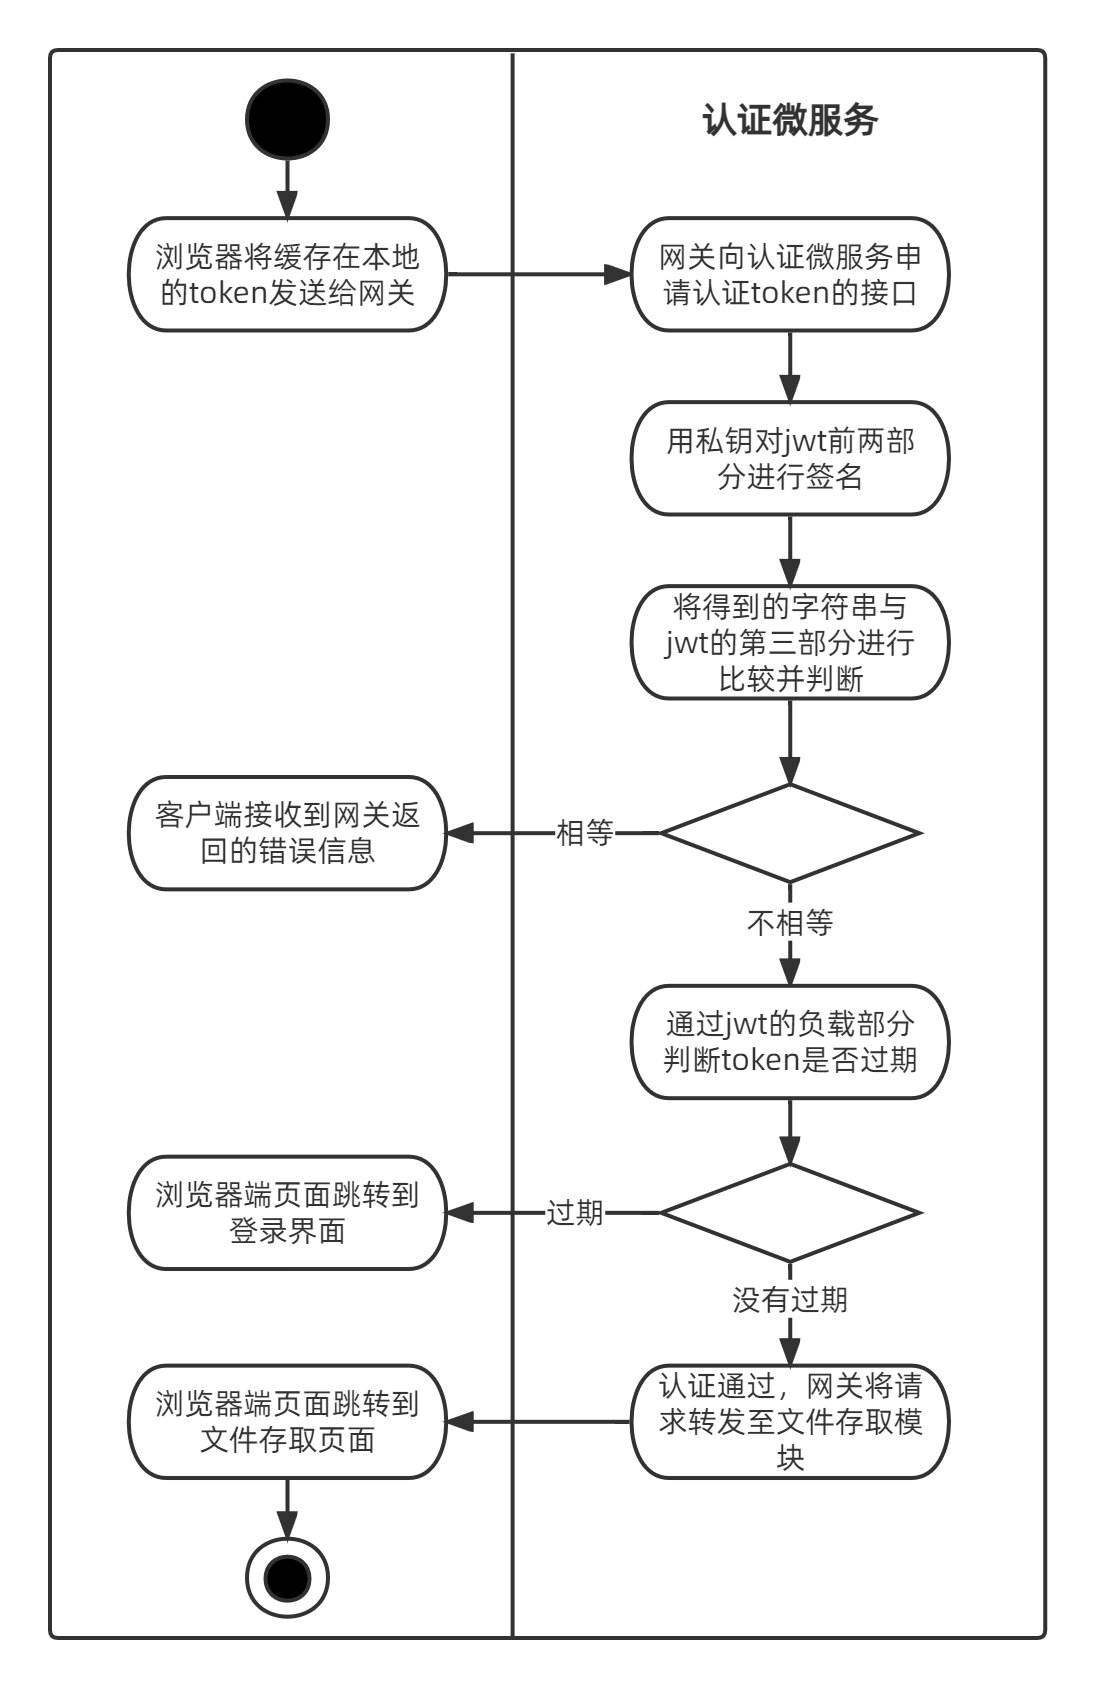
\includegraphics[width=0.7\textwidth]{my_figures/chapter4/认证令牌活动图.png}
%     \caption{认证令牌活动图}
%     \label{fig:认证令牌活动图}
% %     \note{注:图注的内容不宜放到图题中。}
% \end{figure}

\subsection{权限控制模块}

\begin{figure}[h]
    \centering
    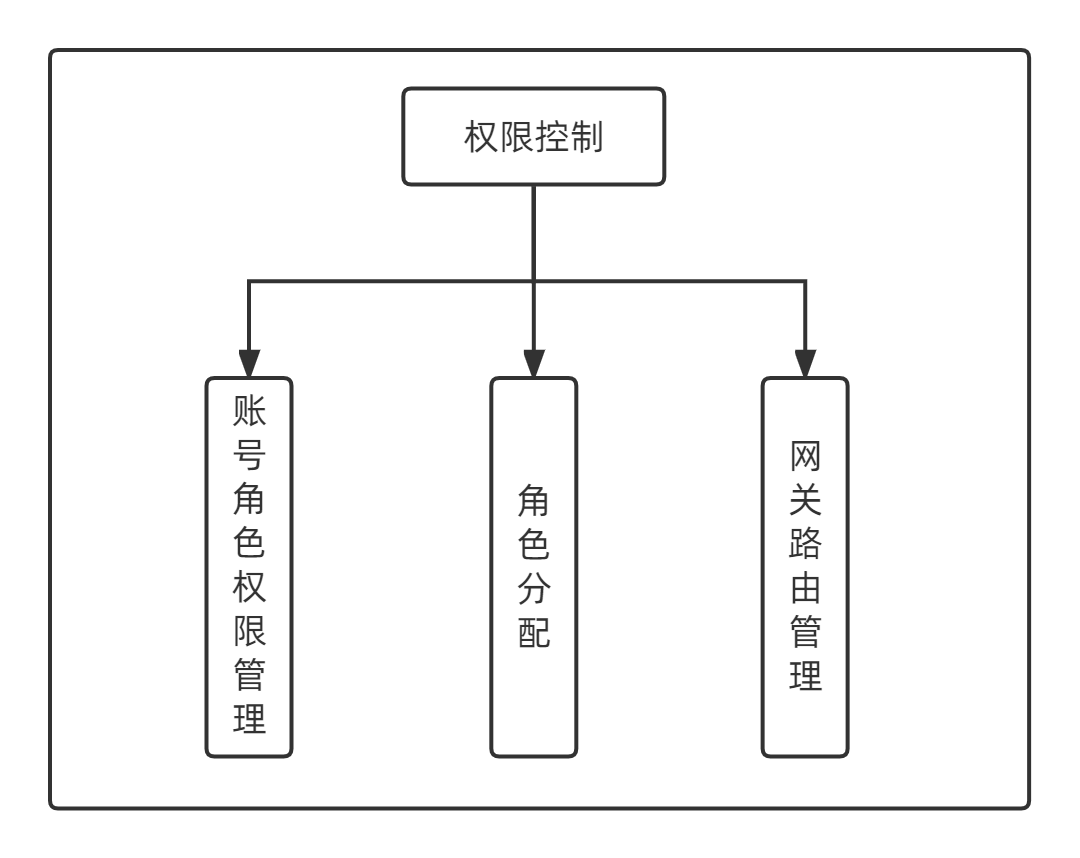
\includegraphics[width=0.5\textwidth]{my_figures/chapter4/权限控制模块功能结构图.png}
    \caption{权限控制模块功能结构图}
    \label{fig:权限控制模块功能结构图}
%     \note{注:图注的内容不宜放到图题中。}
\end{figure}

权限控制模块的主要功能是系统管理员用来管理的角色、权限和网关路由,以及控制整个微服务的入口。

权限控制模块主要包括权限管理、角色管理、请求转发与鉴权、
网关路由管理四个子功能模块。权限管理、角色管理主要负责对角色和权限的信息进行管理和分配,请求转发与鉴权模块的主要功能是为整个系统的安全性提供保
护,因为网关会进行各种安全方面的校验,整个操作系统把网关的所有接口都当做唯一的入口即可。而网关路由管理则主要负责对经过网关路由的信息进行管理。
权限控制模块的功能结构图如图\ref{fig:权限控制模块功能结构图}所示。




(1)权限管理

权限管理子模块负责权限的创建、删除、修改、查询以及分配,这里的权限实际上对应于每一个功能接口,即用户是否有权限访问某个功能接口进行相关操作,
拥有某接口的访问权限本质上就是拥有其访问路径,角色的权限列表中存储的内容就是该角色可访问的路径。所谓权限分配,即将权限与角色进行绑定,在角色
的权限列表中加入某接口的访问路径,则该角色拥有了访问该功能接口的权限,则属于该角色的用户也同样拥有了该权限。由于权限管理的活动图与角色管理的
活动图十分类似,故此处可参考角色管理的活动图\ref{fig:角色管理活动图}。
% 权限管理活动图如图\ref{fig:权限管理活动图}所示。

% \begin{figure}[h]
%     \centering
%     \includegraphics[width=0.7\textwidth]{my_figures/chapter4/权限管理活动图.png}
%     \caption{权限管理活动图}
%     \label{fig:权限管理活动图}
% %     \note{注:图注的内容不宜放到图题中。}
% \end{figure}

(2)角色管理

角色管理子模块主要包含角色的查询与分配,由于本系统默认只有系统管理员、企业管理员和普通用户这三种角色,后面的迭代版本中也不会考虑扩充新的角色,
所以不支持新角色的创建,当然也不允许修改和删除系统默认的角色。角色分配系统主要负责把用户、权限和角色捆绑在一起,给用户绑定一个角色,就等于为员工
设置了一种职务,将权限与角色进行绑定,就等于为职位授予了相应的权力。为保护这两个关联关系,系统分别设计了用户角色关联表和角色权限关联表。用户角色
关联表的记录主要包含用户ID和角色ID两部分,角色权限关联表中的记录则主要包含角色ID和权限ID两部分。系统管理员可能会同时将角色同用户和权限进行绑定
或者解绑,在实现时必须对这种操作实施数据库的事务管理,一旦在事务处理的过程中出现了出错,就可以及时地对操作进行回滚。角色管理活动图如图
\ref{fig:角色管理活动图}所示。

\begin{figure}[h]
    \centering
    \includegraphics[width=0.7\textwidth]{my_figures/chapter4/角色管理活动图.png}
    \caption{角色管理活动图}
    \label{fig:角色管理活动图}
%     \note{注:图注的内容不宜放到图题中。}
\end{figure}

(3)网关鉴权

在微服务架构中,请求转发是指接收到一个请求后,将其转发给下一个处理节点。当系统收到一个操作请求时,会按照设定的路由信息转发到指定的微服务,根据
系统微服务的划分一共设置了五个网关路由项,路由项分别由不同的前缀字段组成,注册认证微服务对应的路由项为/Oauth,权限控制微服务对应的路由项为
/Perm,策略控制微服务对应的路由项为/policyweb,文件存取微服务对应的路由项为/fileweb,系统监控微服务对应的路由项为/systemweb。

\begin{figure}[h]
    \centering
    \includegraphics[width=0.7\textwidth]{my_figures/chapter4/网关鉴权活动图.png}
    \caption{网关鉴权活动图}
    \label{fig:网关鉴权活动图}
%     \note{注:图注的内容不宜放到图题中。}
\end{figure}

系统将用户请求中的前缀与路由项进行对比以决定转发给对应的微服务,如果是转发至策略控制、文件存取和系统监控这三个微服务的请求,系统会使用过滤器对
这些请求进行过滤。网关会在过滤器中调用认证令牌子模块的接口来检查 token 的正确性,如果 token 检查通过,则会调用权限管理模块中的接口。权限管理
模块根据token中的用户名来获取用户的权限列表,该权限列表中包含了用户可访问的路径。然后,过滤器会查找用户权限列表来判断用户请求中的URI是否存在
于该列表中。如果该路径存在,则说明用户拥有访问该接口的权限,否则没有访问权限。在没有权限的情况下,过滤器会向前端返回错误信息。这种设计保证了
只有具有相应权限的用户才能够访问特定的接口,从而提高了系统的安全性。网关鉴权活动图如图\ref{fig:网关鉴权活动图}所示。



\subsection{策略控制模块}

策略控制模块主要负责对注册在存储服务器上的用户、分组和访问策略进行管理。策略控制模块主要包含四个子模块,分别是用户管理子模块,分组管理子模块,策略管理子模块和
策略分配子模块。用户管理子模块主要负责对存储用户的相关数据信息进行管理,分组管理子模块主要负责对存储分组的相关数据信息进行管理,策略管理子模块主要负责对访问策
略的相关数据信息进行管理,策略分配主要负责将策略与用户、策略与分组进行关联,处理这三者之间的分配关系。策略控制模块功能结构如图\ref{fig:策略控制模块功能结构图}
所示。

\begin{figure}[htb]
    \centering
    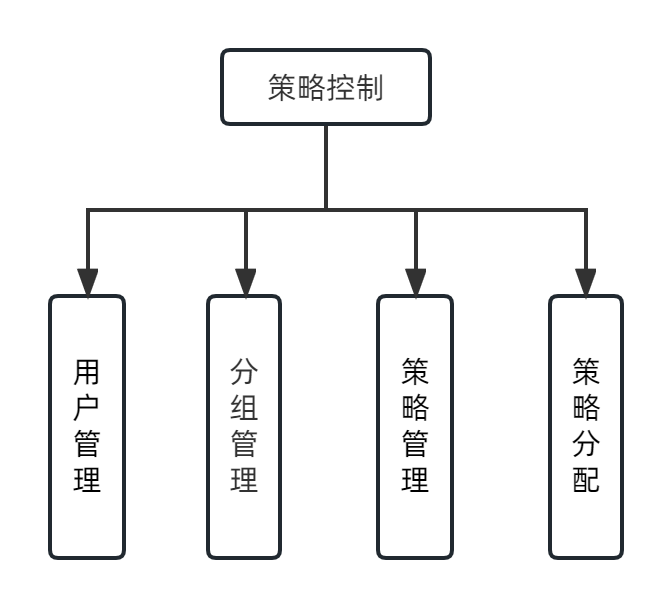
\includegraphics[width=0.5\textwidth]{my_figures/chapter4/策略控制模块功能结构图.png}
    \caption{策略控制模块功能结构图}
    \label{fig:策略控制模块功能结构图}
%     \note{注:图注的内容不宜放到图题中。}
\end{figure}

(1) 用户管理

用户管理主要负责对存储服务器用户账号信息进行数据管理。可以对用户进行增加、删除、修改、查看和禁用操作。用户的信息主要包括用户名、密码、邮箱、
申请容量、已用容量等信息。当需要创建用户时,管理员通过界面输入用户的信息,系统需要对密码进行加密存储,最后将用户信息保存到数据库中。同时,在
对象存储服务器上也会同步创建一个同名的账号。用户信息中申请容量和已用容量等信息都是通过存储服务器获取,因此,当管理员进行修改、删除、查询等操作
时都会同时从数据库和存储服务器中获取数据。用户的权限将由用户所属的角色决定,在权限控制模块中角色和权限会进行绑定,新创建的用户在选择角色时就
已经确定了所拥有的权限了。

当系统进行用户管理的相关操作时,相关操作请求会调用网关鉴权微服务接口,查找用户权限列表来判断用户请求中的URI是否存在于该列表中。如果该路径
存在,则说明用户拥有访问该接口的权限,否则没有访问权限。如果没有访问权限,用户会在前端页面上收到无访问权限的提示,如果有权限,系统会与存储服务
客户端AliIO-Cli建立连接,调用客户端AliIO-Cli提供的用户管理相关API接口,由客户端将请求发送给存储服务器节点。存储服务器节点将完成状态或查询信息反馈给
客户端AliIO-Cli,然后系统调用AliIO-Cli提供的相关API取回状态或查询信息,并在前端页面进行展示。用户管理活动图如图\ref{fig:用户管理活动图}所示。

\begin{figure}[htb]
    \centering
    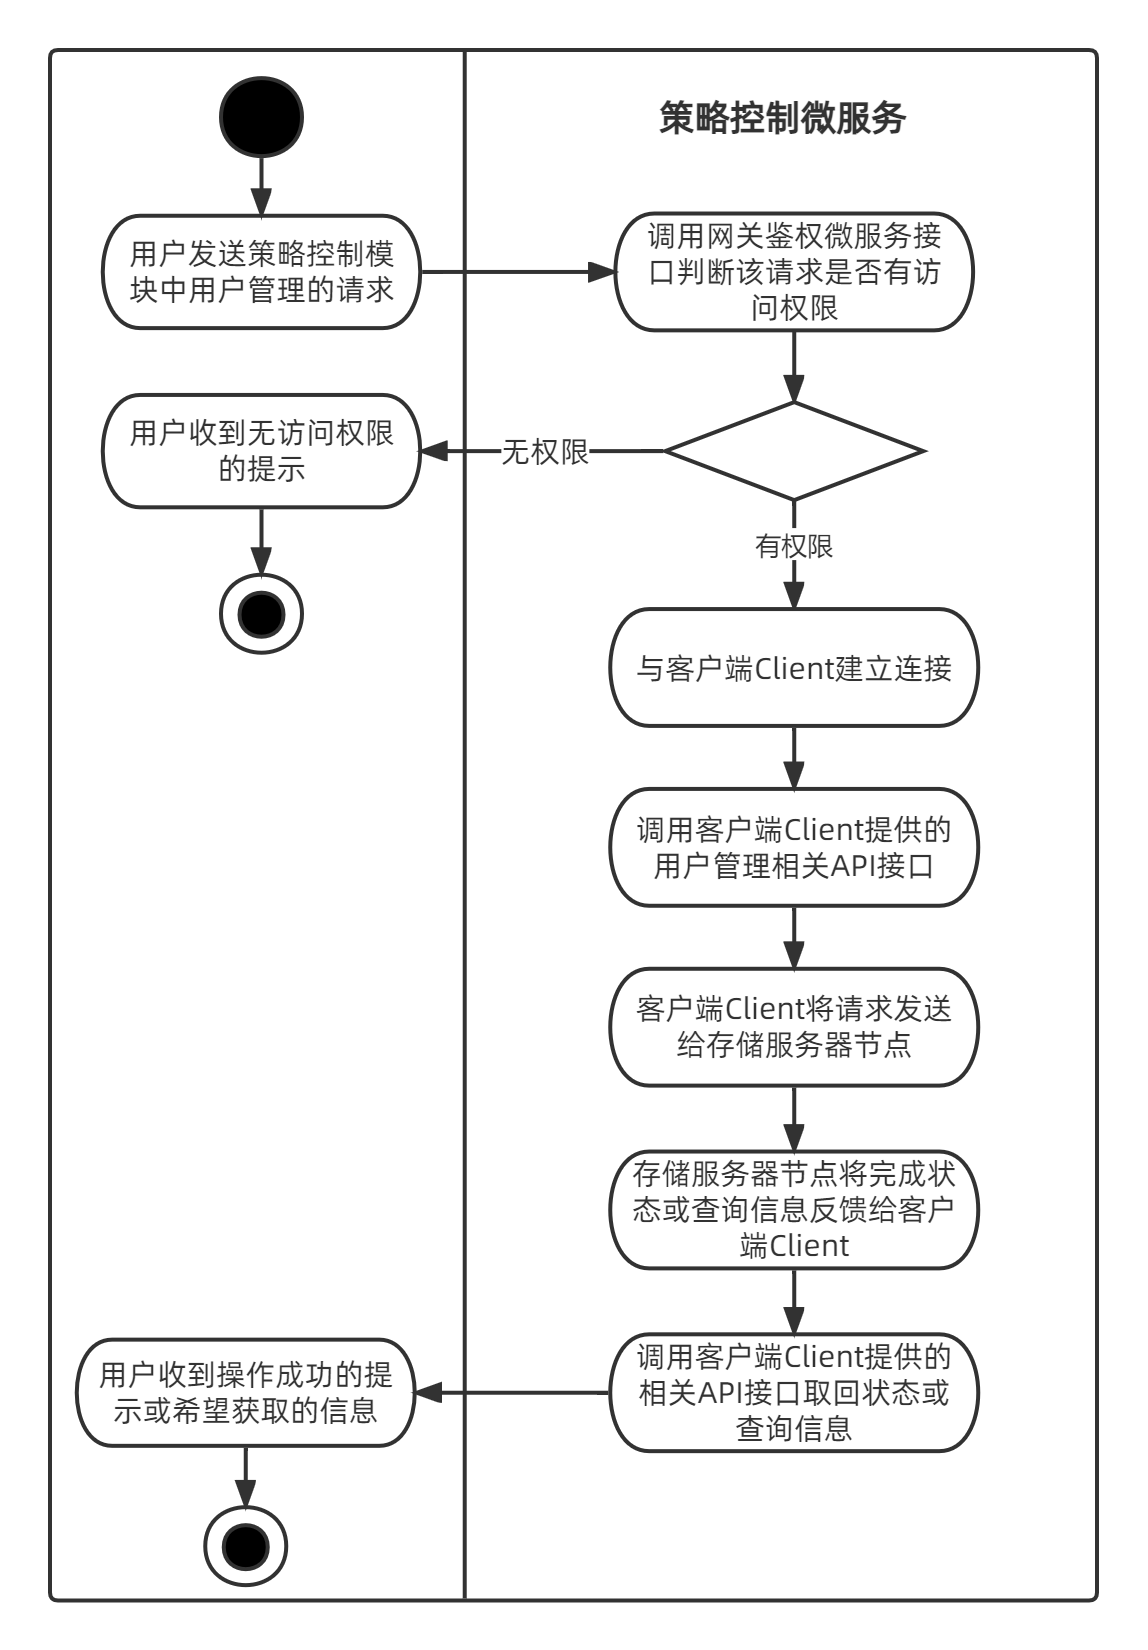
\includegraphics[width=0.7\textwidth]{my_figures/chapter4/用户管理活动图.png}
    \caption{用户管理活动图}
    \label{fig:用户管理活动图}
%     \note{注:图注的内容不宜放到图题中。}
\end{figure}

% (2) 分组管理

% 分组管理主要负责存储服务器分组信息进行数据管理。可以对分组进行增加、删除、修改、查看和禁用操作。存储服务器分组主要包括分组名称、访问策略、是否禁用和创建时间
% 等信息。当系统发出对分组管理模块的使用申请时,首先会使用网关鉴权微服务进行鉴权,如果没授权,会向前端反馈错误的信息,如果有授权,则与客户端AliIO-Cli建立连接,并
% 调用客户端AliIO-Cli提供的API接口,由客户端AliIO-Cli将请求发送给存储服务器节点,待存储服务器处理结束后,会将完成状态或查询信息反馈给客户端AliIO-Cli,管理系统调用客户
% 端AliIO-Cli提供的API取回状态或查询信息,并反馈给前端。分组管理活动图与用户管理活动图十分类似,可参考用户管理活动图\ref{fig:用户管理活动图}。

% \begin{figure}[htb]
%     \centering
%     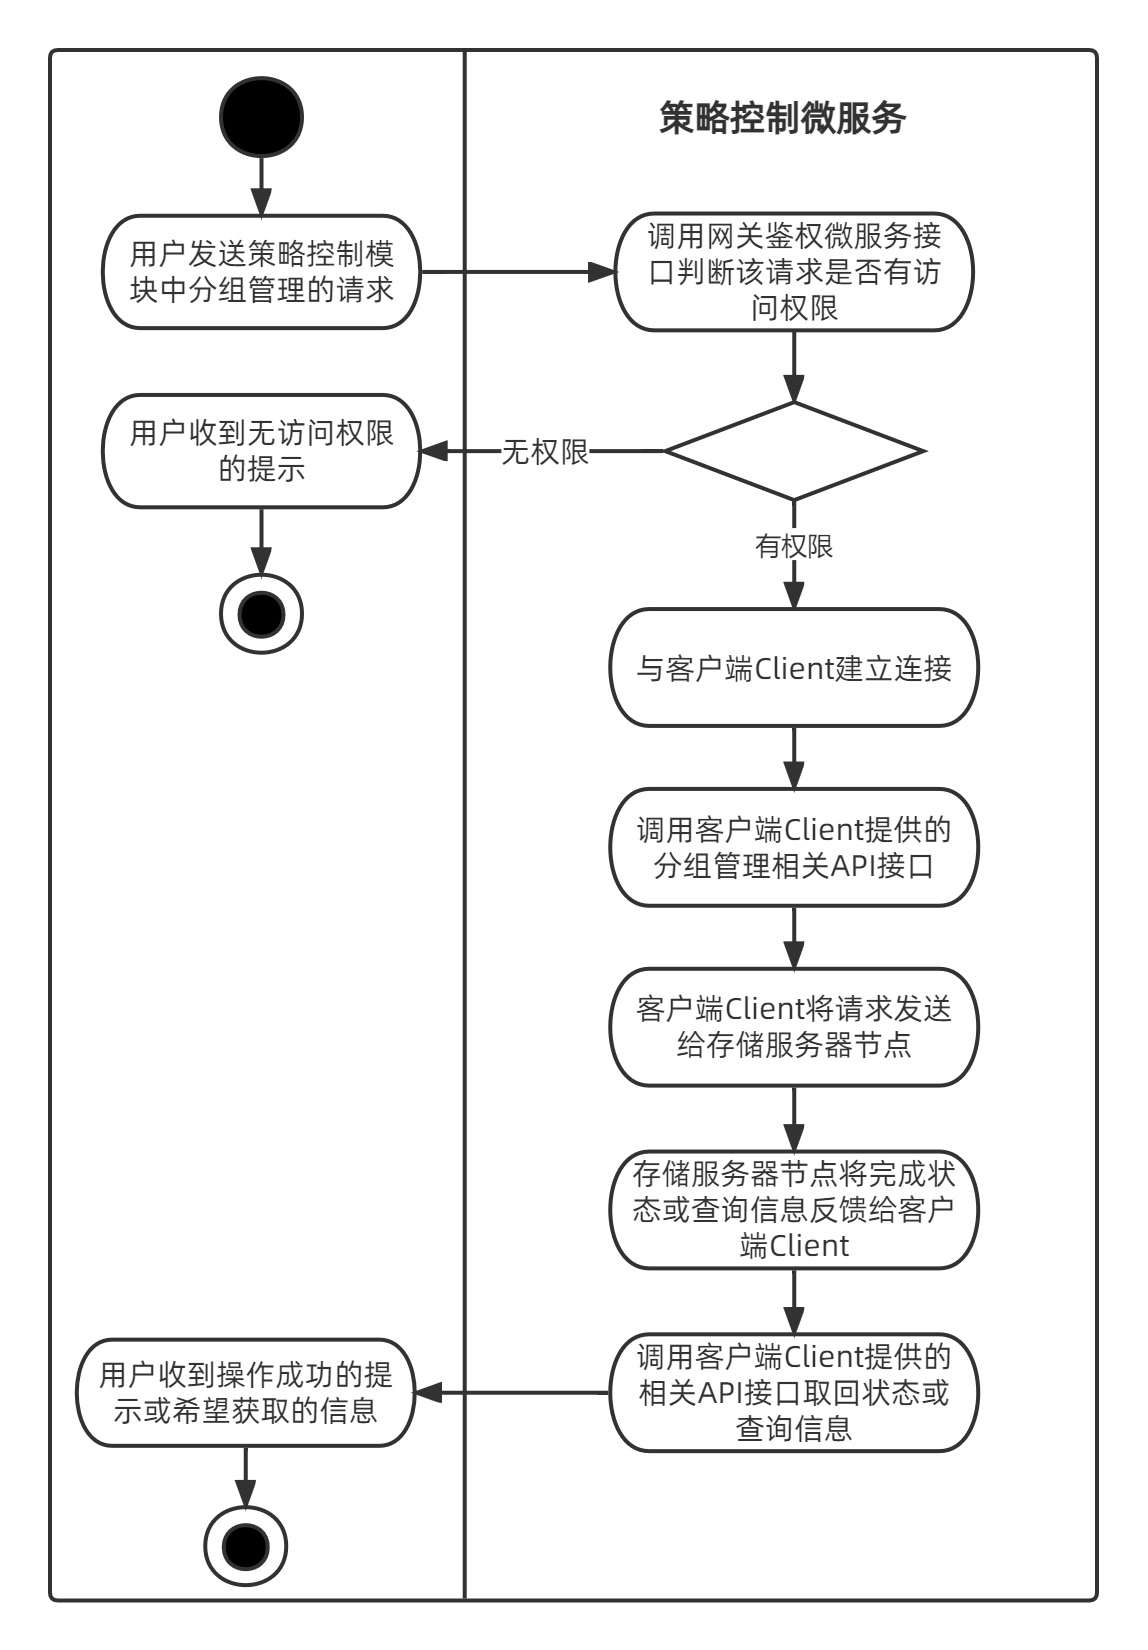
\includegraphics[width=0.8\textwidth]{my_figures/chapter4/分组管理活动图.png}
%     \caption{分组管理活动图}
%     \label{fig:分组管理活动图}
% %     \note{注:图注的内容不宜放到图题中。}
% \end{figure}

(2) 策略管理

策略管理主要负责存储服务器访问策略信息进行数据管理。可以对策略进行增加、删除、修改、查看操作。访问策略主要是针对用户和分组在访问其他用户的Bucket和文件时进行
权限限制,系统已经内置了几种常用的访问策略, 系统中的策略主要分为Bucket访问策略和用户访问策略。
\begin{figure}[htb]
    \centering
    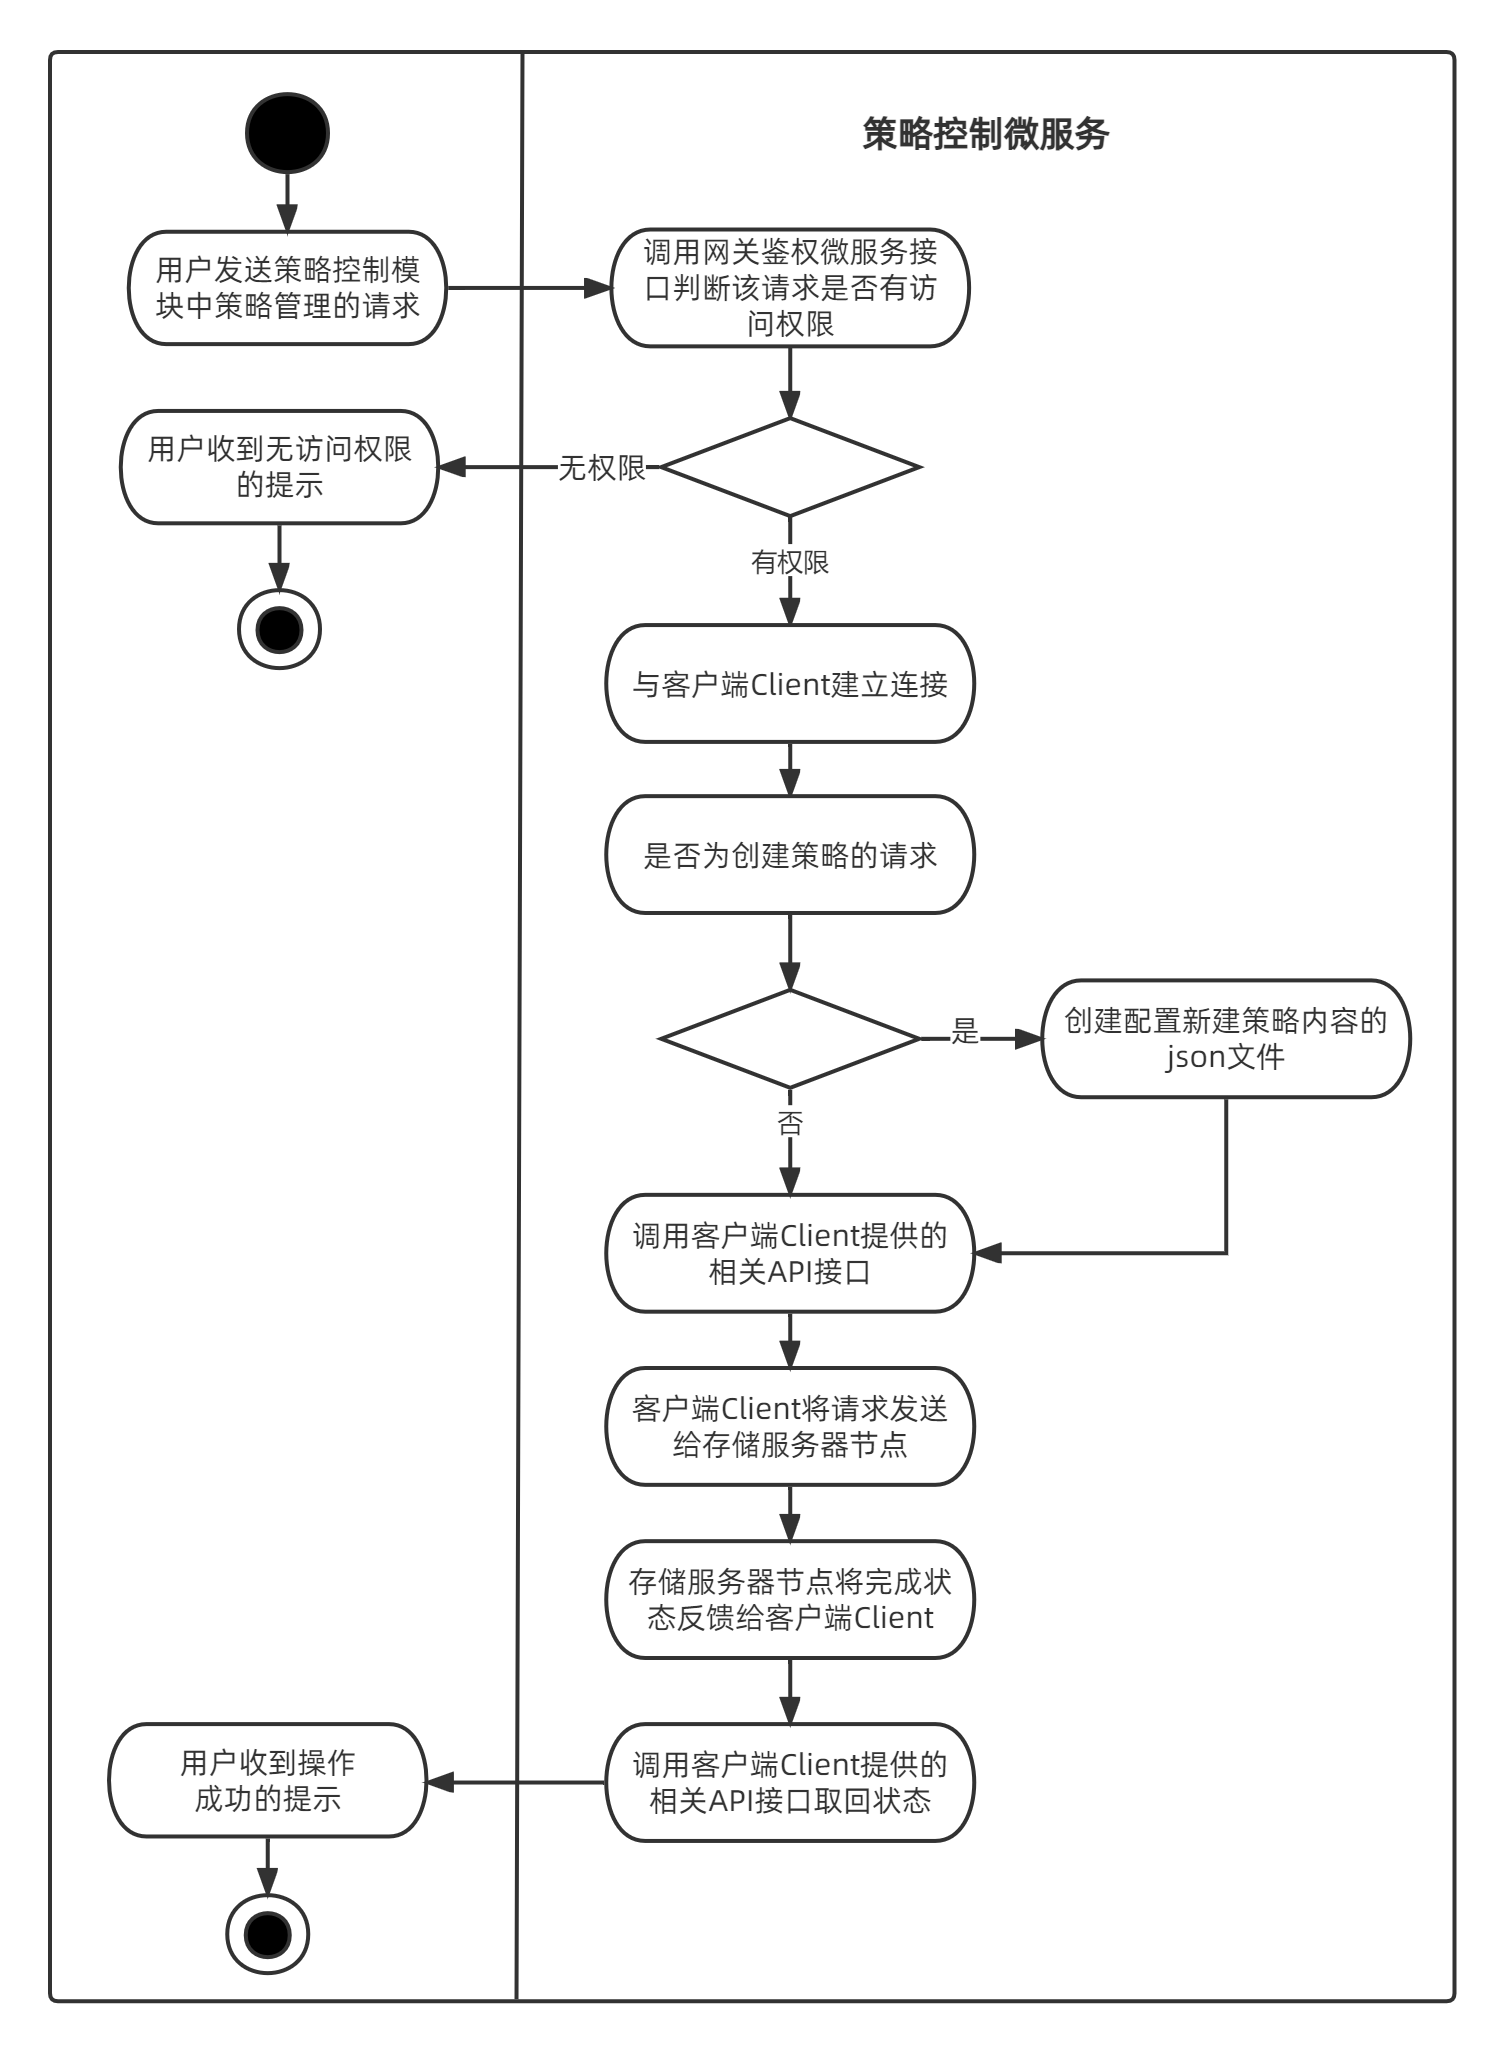
\includegraphics[width=0.7\textwidth]{my_figures/chapter4/策略管理活动图.png}
    \caption{策略管理活动图}
    \label{fig:策略管理活动图}
%     \note{注:图注的内容不宜放到图题中。}
\end{figure} 
Bucket访问策略主要有public、custom和private
三种,系统内置的用户访问策略主要有五种,分别是控制台管理员(consoleAdmin)策略、诊断(diagnostics)策略、只读(readonly)策略、
读写(readwrite)策略和只写(writeonly)策略。

当设置Bucket的使用方式是public后,用户必须不通过任何验证才能进行使用资源;当设置Bucket的访问
方式是custom后,Bucket的最终访问策略由具体的用户访问策略决定,用户访问策略可以是系统内定的策略,如只读(readonly)策略、读写(readwrite)策
略和只写(writeonly)策略,也可以是自定义的访问策略;当设置Bucket的访问策略为private时,用户未经授权不能进行任何操作,所有用户访问策略失效。
因此,Bucket的访问策略权限要大于用户访问策略。

当管理员在执行策略管理的相关操作时,如果是创建新的策略,那么管理员需要需要配置相关的策略模板文件,该文件包含新策略的实际内容。该文件主要含有Version、
Statement、Effect、Principal、Action、Resource等配置项,管理员可根据需要自定义该文件的内容。当删除某个自定义的策略时,如果
有用户或分组正在使用该策略,则删除该策略后,用户或分组的策略会自动变为默认的策略。策略管理活动图如图\ref{fig:策略管理活动图}所示。

(3) 策略分配




策略分配主要负责将预定义的策略分配给特定的用户或用户组,以控制他们对存储桶和对象的访问权限。当管理员登录到管控平台,进入策略管理页面,管理员
选择一个或多个用户或用户组,然后将预定义的策略分配给他们。

\begin{figure}[h]
    \centering
    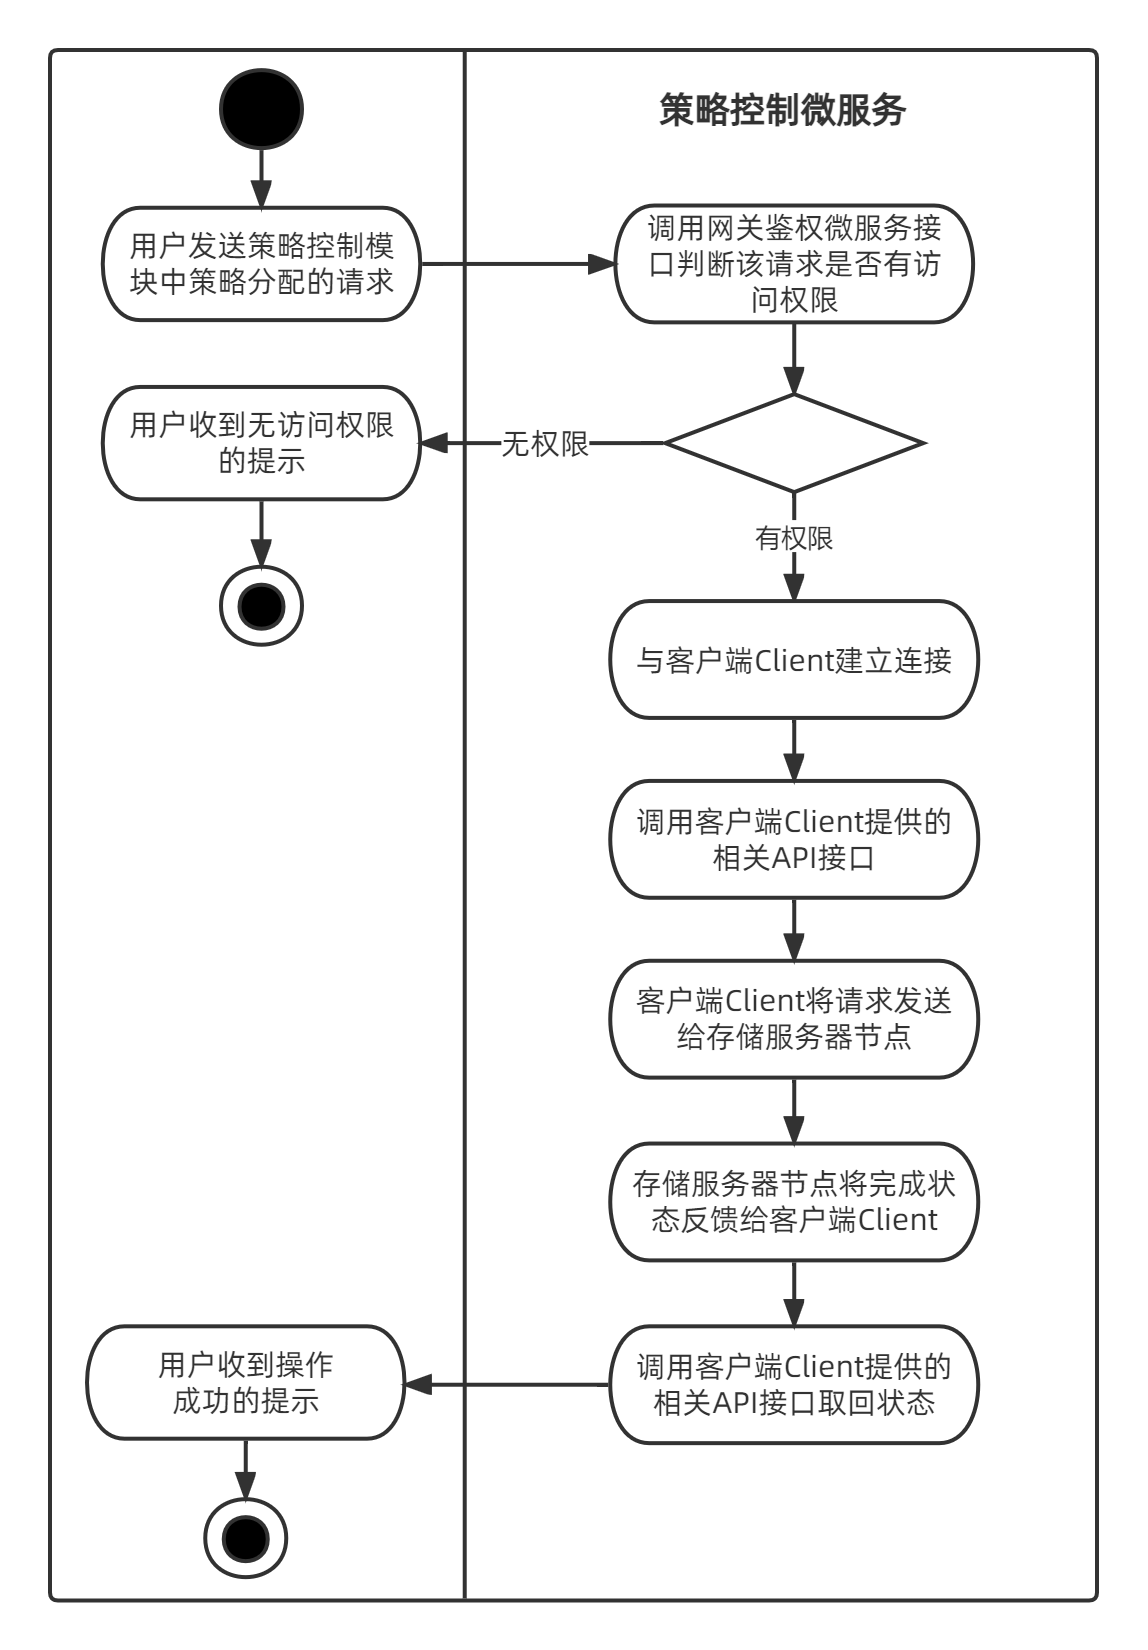
\includegraphics[width=0.7\textwidth]{my_figures/chapter4/策略分配活动图.png}
    \caption{策略分配活动图}
    \label{fig:策略分配活动图}
%     \note{注:图注的内容不宜放到图题中。}
\end{figure}

如果管理员想要更加细粒度地控制用户的访问权限,可以在分配策略的时候设置一些参数,
例如:存储桶的访问权限、对象的访问权限、访问时间等。管理员保存分配的策略,管控平台会自动将该策略的授权信息同步到后端的对象存储系统中。管理员
可以同时对用户或用户组分配策略,如果一个用户属于某个分组,如果二者的策略不同,若分组的策略比用户的策略更加严格,则对用户的策略进行升级,否则,
用户仍保持自己的策略不变。策略分配活动图如图\ref{fig:策略分配活动图}所示。



\subsection{文件存取模块}

% 文件存储模块是本系统最核心的模块,也是普通用户访问最频繁的模块,该模块主要分为四个子模块,分别是桶管理子模块、文件上传子模块、文件下载子模块和文件删除子模块。
% 文件存取模块功能结构图如图\ref{fig:文件存取模块功能结构图}所示。
\begin{figure}[h]
    \centering
    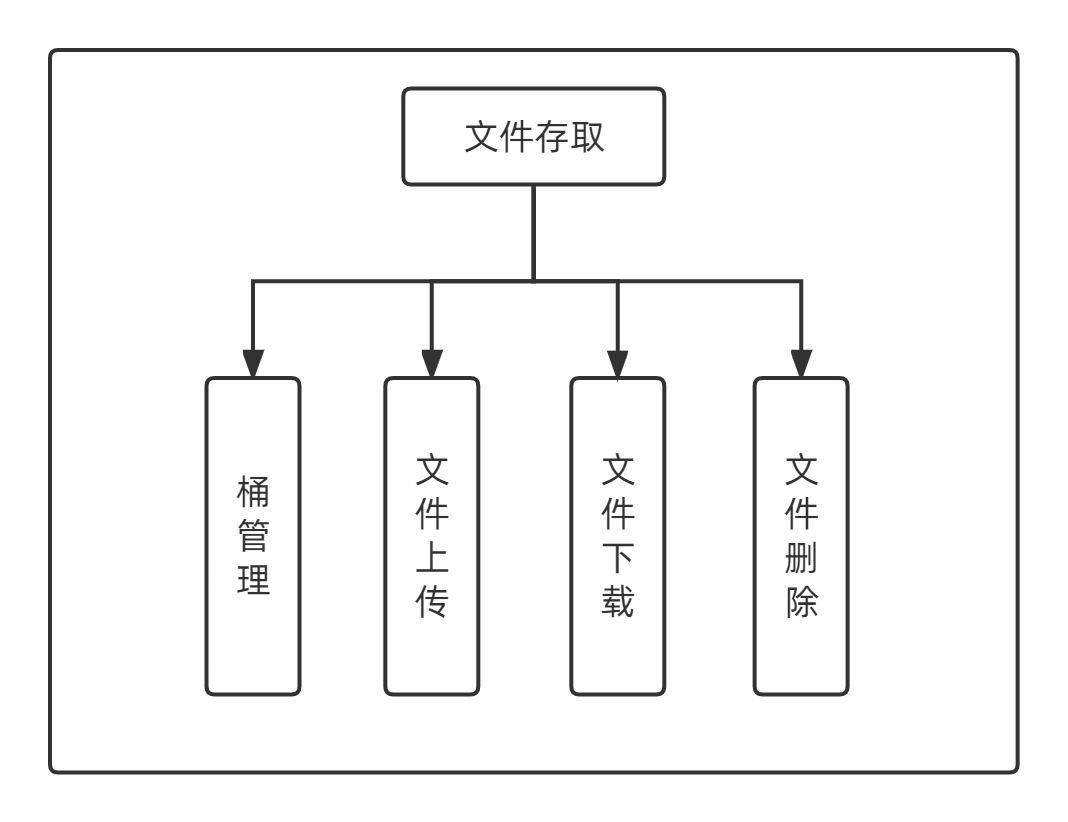
\includegraphics[width=0.5\textwidth]{my_figures/chapter4/文件存取模块功能结构图.png}
    \caption{文件存取模块功能结构图}
    \label{fig:文件存取模块功能结构图}
%     \note{注:图注的内容不宜放到图题中。}
\end{figure}

文件存储模块是本系列中最基础的功能,同时也是普通用户访问最常见的功能,该模块主要包括了四大子模块,分别为桶管理子模块、
文件上传子模块、文件下载子模块和文件共享子模块。文件存取模块功能的结构图如图\ref{fig:文件存取模块功能结构图}所示。



(1) 桶管理



桶管理模块主要负责对用户的存储桶进行管理。桶管理功能通常包括创建桶、删除桶、修改桶属性、查看桶列表、查看桶属性等操作。但操作的前提是用户拥有对
应的访问策略,比如用户对桶的访问策略是只读,那么该用户将只能对桶进行查看,无法对其中的文件进行修改、删除等其他操作。
\begin{figure}[htb]
    \centering
    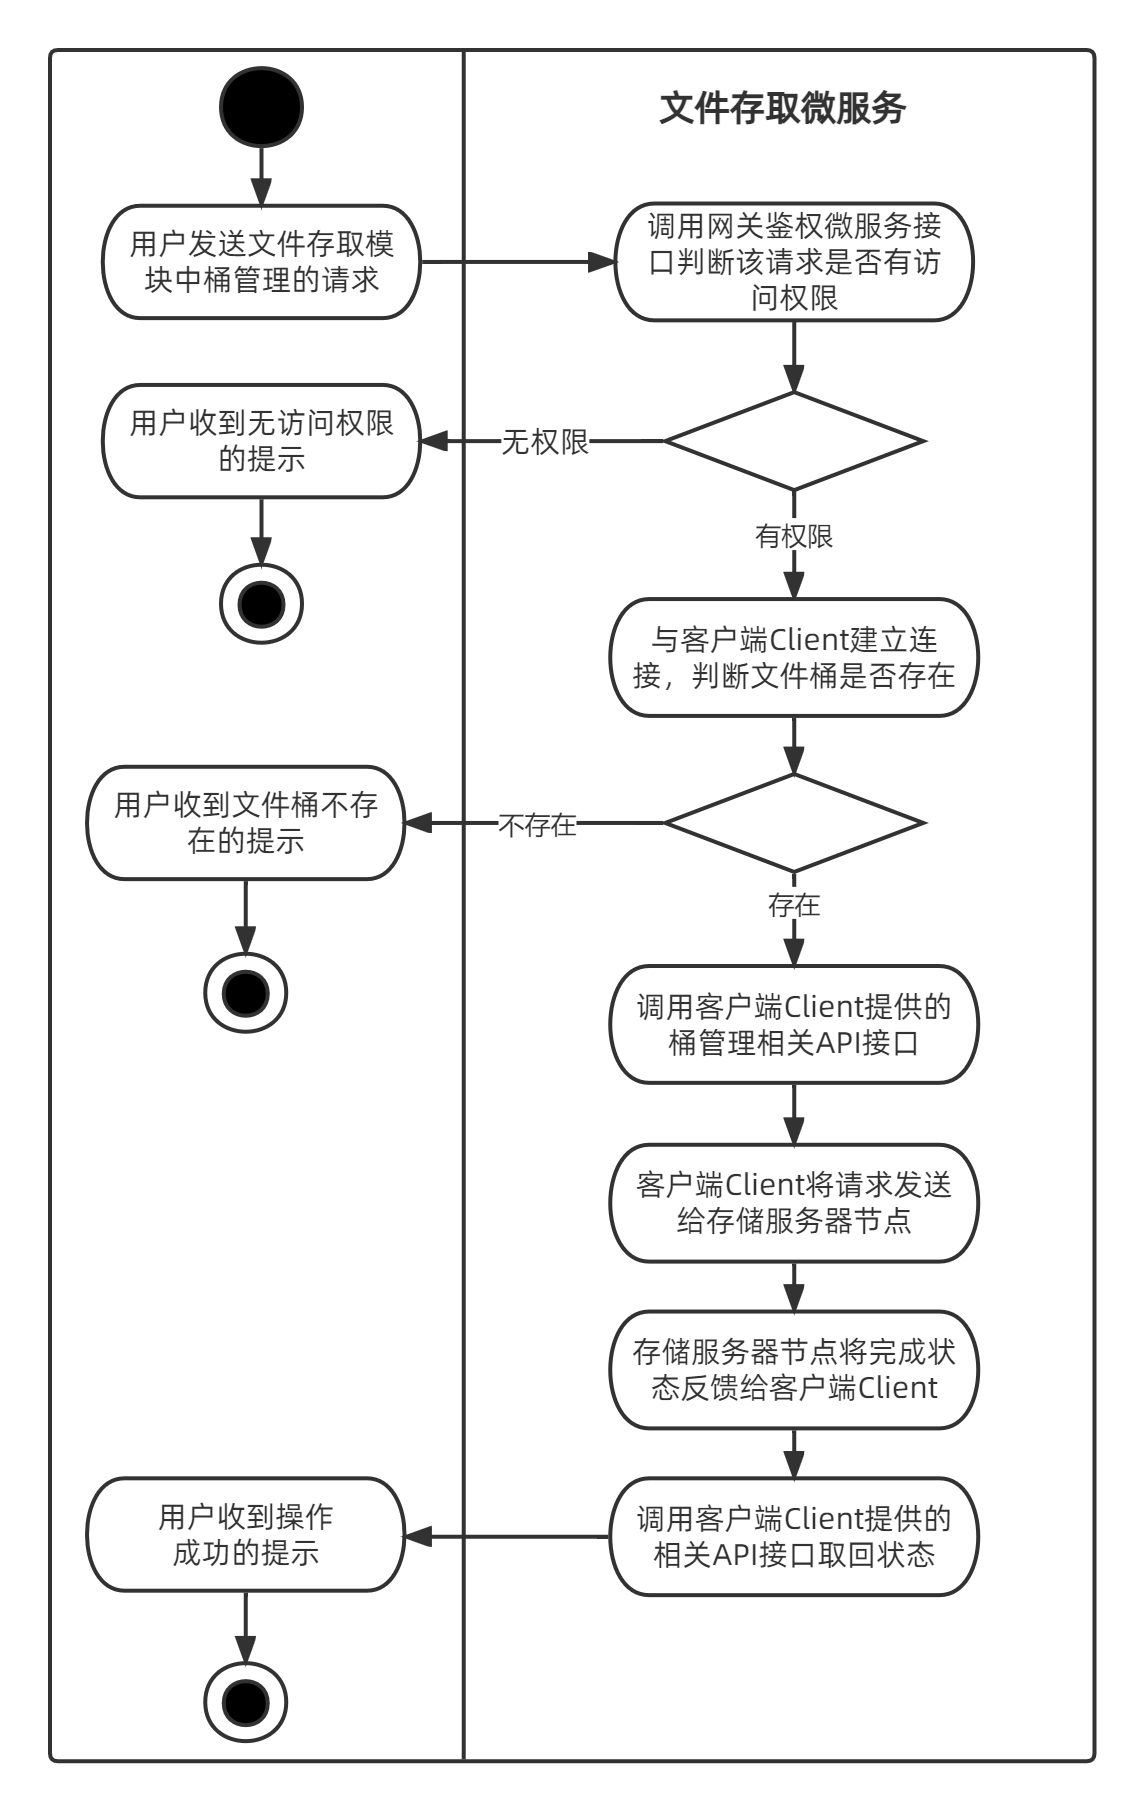
\includegraphics[width=0.7\textwidth]{my_figures/chapter4/桶管理活动图.png}
    \caption{桶管理活动图}
    \label{fig:桶管理活动图}
%     \note{注:图注的内容不宜放到图题中。}
\end{figure}

用户在系统中创建新的桶时,
要填写唯一的名称、访问权限、存储类别等属性。创建桶时,需要根据需求确定桶的存储区域、容量、生命周期等设置,以便后续的文件上传、访问和管理。对桶
进行删除操作时,删除操作会将桶内所有文件删除,所以删除前需要用户确认。删除桶时,需要先删除桶内所有的文件,然后再执行删除桶的操作。用户可修改桶
的各种属性,如桶名称、访问权限、存储类别、生命周期等。修改桶属性时需要注意,修改某些属性可能会对桶内已有的文件产生影响,需要用户慎重处理。用户
还可以查看桶列表和桶属性,可根据桶名称、存储区域等条件进行搜索和过滤,快速定位目标桶。

还可以查看指定桶的详细属性信息,包括桶名称、访问权限、
生命周期、当前使用量、文件数量等。还支持用户查看桶内的文件列表、访问日志等信息,方便监控和管理。在用户执行上述除创建以外的操作时,都需要先判断
桶是否存在,如果桶不存在,前端页面将会显示文件不存在的提示;如果桶存在,则流程会继续往下进行,和对象存储系统服务器进行交互。桶管理活动图如图
\ref{fig:桶管理活动图}所示。




(2) 文件上传

\begin{figure}[htb]
    \centering
    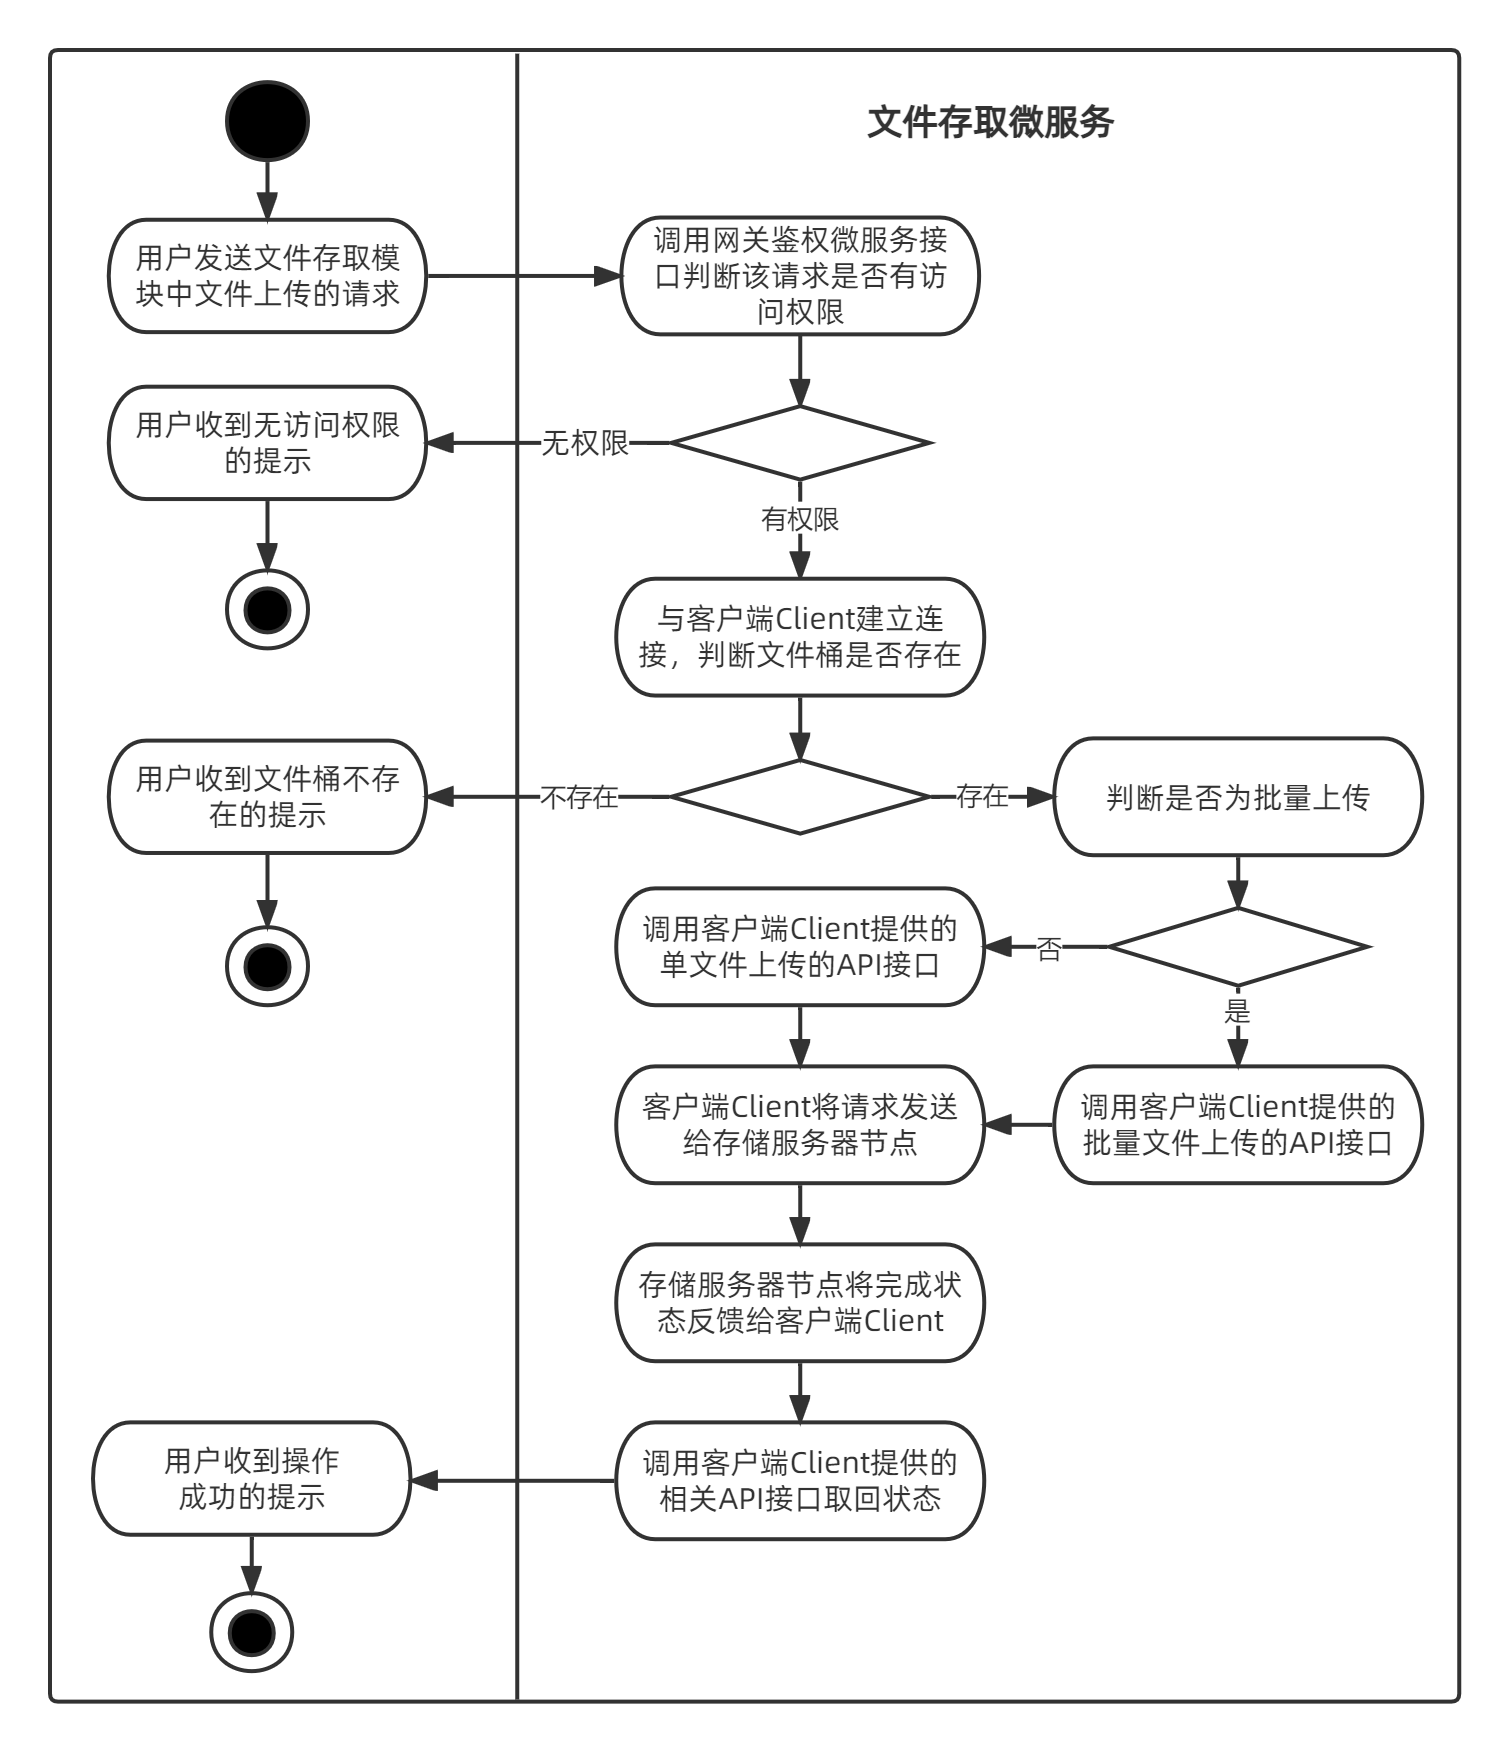
\includegraphics[width=0.7\textwidth]{my_figures/chapter4/文件上传活动图.png}
    \caption{文件上传活动图}
    \label{fig:文件上传活动图}
%     \note{注:图注的内容不宜放到图题中。}
\end{figure}

% 文件上传模块主要负责将用户的文件上传至数据存储服务器中,支持上传多种不同类型的文件,也可以进行多文件批量上传,
文档上传功能主要是将用户的文件上传至对象存储服务器上。当用户进行文件上传时,在上传前需要进行鉴权操作,确保上传者具备相应的权限。同时,需要对上
传的文件进行一些安全性和完整性的检查,如文件类型、大小等限制以及MD5等校验码的生成和校验。上传成功后,需要将文件存储在分布式对象存储系统中,并
返回文件的URL地址供后续的访问使用。系统支持用户提交各种不同形式的文档,同时能够实现多文件批量上传对文件的大小限制也很宽松,一般情况下,只要文件
大小不超过1T,都可以正常的完成上传。在上传过程中前端可以看到文件上传的实时进度,如果遇到网络波动或断线,前端会有相应的反馈通知,网络故障时,系
统会暂停文件的上传。文件上传活动图如图\ref{fig:文件上传活动图}所示。



(3) 文件下载


文件下载功能主要是把文件从对象存储服务器下载到用户本地。对于文件下载,同样需要进行鉴权操作,确保下载者具备相应的权限。一般用户通过Web界面或者
API接口进行文件下载操作,系统需要根据文件URL地址从分布式对象存储系统中获取对应的文件,并将文件返回给用户。在返回文件时,还需要进行一些安全性和
完整性的检查,如文件大小、MD5等校验码的校验。和文件上传一样,也支持多文件批量下载,在下载过程中前端可以看到文件下载的实时进度,如果遇到网络波动或
断线,前端会有相应的反馈通知,网络故障时,系统会暂停文件的下载。整体的操作流程和文件上传类似。文件下载活动图与文件上传活动图十分类似,此处可参考
文件上传活动图\ref{fig:文件上传活动图}。

% \begin{figure}[htb]
%     \centering
%     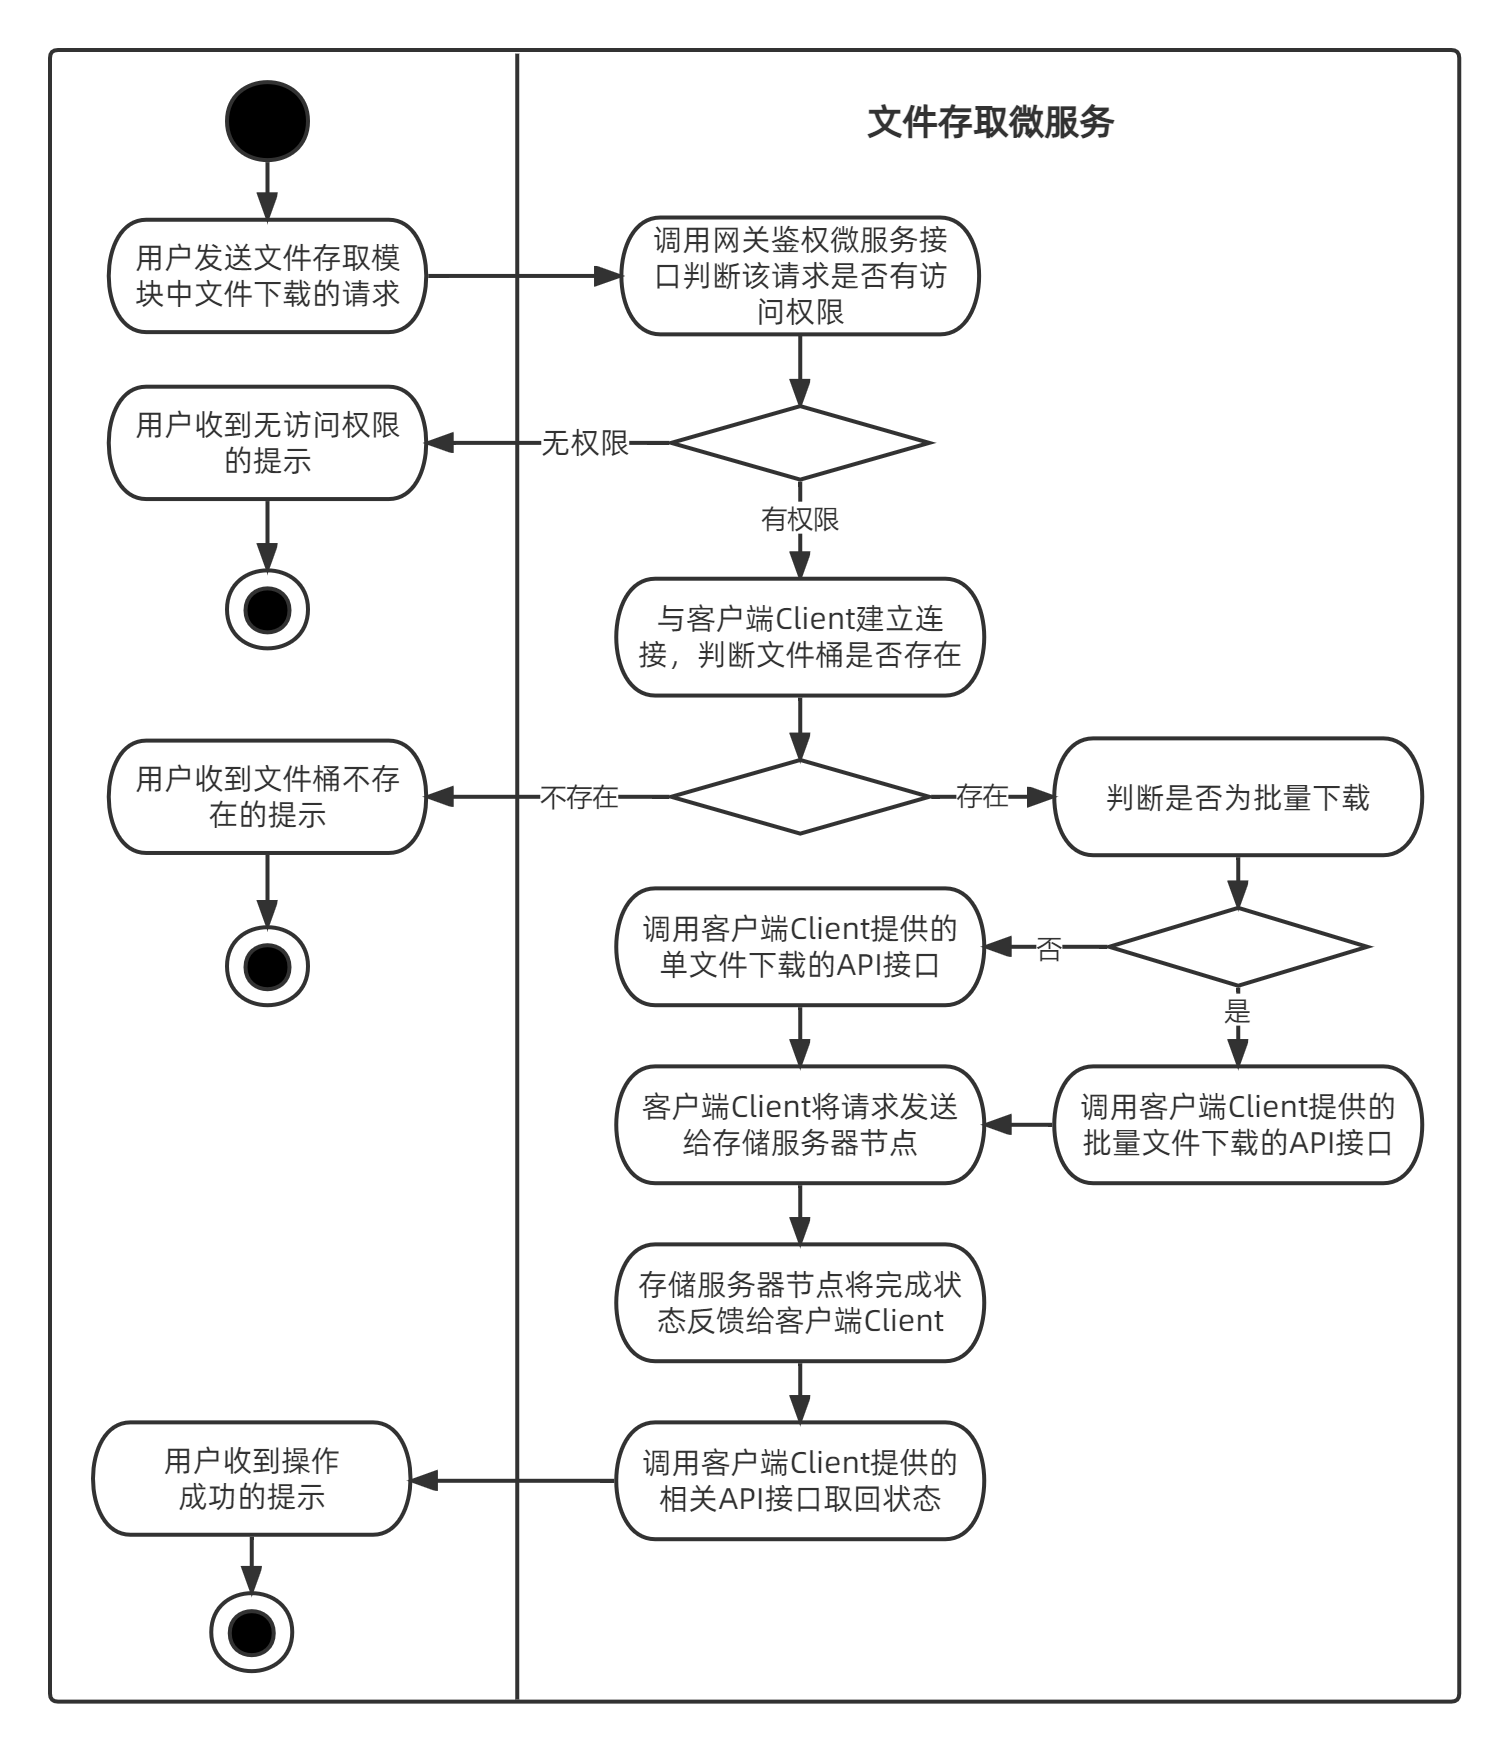
\includegraphics[width=0.7\textwidth]{my_figures/chapter4/文件下载活动图.png}
%     \caption{文件下载活动图}
%     \label{fig:文件下载活动图}
% %     \note{注:图注的内容不宜放到图题中。}
% \end{figure}

% (4) 文件共享

% 文件共享模块主要负责对用户Bucket中的文件进行共享。用户在选中某个文件后,并将其设置为共享,则所有用户均可访问该文件,但文件访问链接是一个
% 临时的共享链接,链接中包含了共享文件的地址、有效期、以及访问密码等信息。用户可以根据自己的需要设置这些参数,然后将链接分享给其他用户。
% 当其他用户或者组织收到共享链接后,需要进行访问授权。授权主要是通过访问密码方式进行。一旦授权通过,用户就可以通过访问
% 共享链接来访问共享文件了。对象存储系统AliIO会根据授权信息来判断用户是否有权访问该文件,如果权限通过,则可以下载或者查看该文件。文件的共享后,其
% 访问策略仍然为文件所属用户设置的策略,任何人无权更改。用户可随时取消文件共享,被用户取消共享或过了有效期的文件将无法访问。对于用户的每一次
% 共享,都会产生一条共享记录,其内容包括共享的文件名、共享的用户、共享的时间等信息。文件共享操作活动图如图\ref{fig:文件共享活动图}所示。

% \begin{figure}[h]
%     \centering
%     \includegraphics[width=0.7\textwidth]{my_figures/chapter4/文件共享活动图.png}
%     \caption{文件共享活动图}
%     \label{fig:文件共享活动图}
% %     \note{注:图注的内容不宜放到图题中。}
% \end{figure}


\subsection{系统监控模块}

\begin{figure}[h]
    \centering
    \includegraphics[width=0.5\textwidth]{my_figures/chapter4/系统监控模块功能结构图.png}
    \caption{系统监控模块功能结构图}
    \label{fig:系统监控模块功能结构图}
%     \note{注:图注的内容不宜放到图题中。}
\end{figure}

系统监控模块主要是对系统运行状态的实时监控、分析和报警,以确保系统运行的稳定性和可靠性。
系统维护模块主要包含三个子模块,分别是状态监控子模块、
记录跟踪子模块和告警通知子模块。只有系统管理员才有该模块的访问权限。系统维护模块的功能结构图如图\ref{fig:系统监控模块功能结构图}所示。


(1)状态监测

% \begin{figure}[h]
%     \centering
%     \includegraphics[width=0.6\textwidth]{my_figures/chapter4/状态监测活动图.png}
%     \caption{状态监测活动图}
%     \label{fig:状态监测活动图}
% %     \note{注:图注的内容不宜放到图题中。}
% \end{figure}


状态监测的主要功能是监测整个存储系统的状态,本系统设置的监控指标有存储桶和对象数量、服务器数量、服务器状态、系统负载、存储容量、吞吐量、响应时间等,
使用监控工具Prometheus进行监控数据
采集和存储,定期对采集的数据进行分析和统计,以便后续数据展示和告警处理。在收集到这些数据后,通过数据可视化工具Grafana将监控数据进行可视化展示,
方便管理员及时了解系统状态,及时发现和解决问题。同时,通过数据分析技术,对数据进行趋势分析、异常检测等,提前发现潜在的问题。



当系统管理员进入系统监测页面时,相应的操作请求首先会通过网关鉴权模块进行权限检查,如果有权限,就会和客户端AliIO-Cli建立连接,调用客户端提供的
查询桶和对象数量、服务器状态、存储容量等相关的API接口,由客户端向对象存储系统AliIO的服务器节点发送命令,通过监控工具Prometheus采集和存储对象
存储服务器相关的状态数据\cite{kongqoji},由数据可视化工具Grafana将监控数据进行可视化展示在页面上\cite{kong2324qoji}。
% 状态监测活动图如图\ref{fig:状态监测活动图}所示。



(2)事件跟踪

事件追踪主要是负责对操作日志、事件日志进行记录和分析,方便系统管理员快速定位和解决问题。在整个管控平台中,日志可以分为两类:系统日志和访问日志。
系统日志记录系统的各种操作和事件,如用户登录、文件上传、权限分配等;访问日志记录用户对文件的访问情况,如文件下载、分享等。针对这两类日志,对象
存储系统管控平台需要提供不同的管理方式。对于系统日志,平台对系统中的各种操作和时间进行收集,并存储到日志数据库中。系统管理员可随时查询日志,并且
系统还提供日志分析功能,会对所有日志进行分析并生成相应的日志报告,让管理员查看系统的运行情况。对于访问日志,平台对用户对文件的访问情况进行收集,
并存储到日志数据库中。系统管理员可根据时间、文件名、用户等条件查询访问日志。同样,系统也会对日志进行分析,并将日志保留一定的时间。



\begin{figure}[htb]
    \centering
    \includegraphics[width=0.6\textwidth]{my_figures/chapter4/记录跟踪活动图.png}
    \caption{事件跟踪活动图}
    \label{fig:记录跟踪活动图}
%     \note{注:图注的内容不宜放到图题中。}
\end{figure}

当系统管理员进入记录跟踪页面时,相应的操作请求首先会通过网关鉴权模块进行权限检查,如果有权限,就会和客户端AliIO-Cli建立连接,调用客户端提供的
日志管理相关的API接口,从日志数据库中取出日志,由对象存储系统AliIO对日志进行分析,并生成相应的日志报告,返回给前端页面。
记录跟踪活动图如图\ref{fig:记录跟踪活动图}所示。



(3)告警通知

告警通知主要负责在系统监测的那些指标出现异常时及时通知管理员或相关负责人,以便快速响应并处理问题,确保系统的稳定性和可靠性。对于系统需要监控的
告警类型,主要就是以状态监测模块中的那些监测指标为主,如磁盘空间不足、系统负载过高、网络连接异常等。系统根据异常类型的紧急程度,定义了不同的告警
级别,如紧急、重要、普通等,以便管理员快速判断和处理问题。当出现告警时,系统会以邮件和短信的形式通知系统管理员\cite{kngqineji}。系统管理员可以在界面上配置告警类
型、级别、通知方式、接收人等信息,还可以去设置触发告警阈值或条件,比如磁盘使用率超过90\%等。系统会记录每一次告警的信息,包括告警类型、级别、时
间、通知方式、接收人、处理结果等,以便后续的跟踪和分析。

当系统监测的指标达到相应的触发条件时,会向系统中设置的接收人发送告警通知,通知的内容包括告警类型标、告警内容、告警级别、发生时间等信息,并将相应的
告警信息存入数据库。告警通知活动图如图\ref{fig:告警通知活动图}所示。

\begin{figure}[htb]
    \centering
    \includegraphics[width=0.6\textwidth]{my_figures/chapter4/告警通知活动图.png}
    \caption{告警通知活动图}
    \label{fig:告警通知活动图}
%     \note{注:图注的内容不宜放到图题中。}
\end{figure}


\section{数据库总体设计}

分布式对象存储系统管控平台需要存储大量的数据信息,这些数据信息包括用户信息、角色信息、权限信息、路由信息、状态信息、日志信息、告警信息等,而且
这些信息也会随着用户的增多而逐渐增加,这些数据无论是对用户还是对系统管理人员都是尤为重要的。因此,良好的数据库设计可以有效的管理这些重要的数据
信息,提高系统的效率和稳定性。结合本系统的需求特点,最终选用MySQL数据库进行后台数据的管理。MySQL是一种关系型数据库管理系统(RDBMS),它是一个
开源的、基于客户端-服务器模型的数据库系统\cite{kn2e2i},大可以处理大量数据和并发用户,同时具有自动故障转移和备份恢复功能,可确保数据的可靠性和完整性。
由于MySQL具有高性能、可靠性、安全性、可扩展性等优点,成为本系统首选的数据库管理系统。

% \subsection{数据库E-R图设计}

在数据库设计过程中,实体-关系图(E-R图)的绘制是不可省略的步骤,它用于描述实体(Entity)和实体之间的关系(Relationship)\cite{kng2eji},该建模工具让开发者
更清晰的理解和梳理数据之间的关系。根据需求分析可知,本系统的实体有用户、角色、权限、策略、存储桶、存储服务器、日志信息、告警信息,各实体之间的
关系(即E-R图)如图\ref{fig:E-R图}所示。

\begin{figure}[htb]
    \centering
    \includegraphics[width=1\textwidth]{my_figures/chapter4/E-R图.png}
    \caption{分布式对象存储系统管控平台E-R图}
    \label{fig:E-R图}
%     \note{注:图注的内容不宜放到图题中。}
\end{figure}

\section{本章小结}

本章主要从分布式对象存储系统管控平台的系统架构作为切入点,对系统进行了详细的分析和介绍。首先,结合系统架构图,介绍了系统的逻辑架构和后端的技术架构
,以及系统各个模块的功能模块设计。然后,根据各个模块的功能结构图和UML活动图,对各个功能模块的设计进行了深入的介绍,包括注册认证模块、权限控制
模块、策略控制模块、文件存取模块、系统监控模块。最后,借助E-R图对数据库表之间的关系进行了说明。本章对分布式对象存储系统管控平台进行了概要设计,
为后面的详细设计提供了依据。